\documentclass[]{sigplanconf}


\pdfpagewidth=8.5in
\pdfpageheight=11in

\usepackage[T1]{fontenc}

\usepackage[utf8x]{inputenc}
\usepackage{cite}
\usepackage{graphicx}
\usepackage{alltt}

%opening
\begin{document}

\conferenceinfo{Erlang'11,} {September 23, 2011, Tokyo, Japan.}
\CopyrightYear{2011}
\copyrightdata{978-1-4503-0859-5/11/09}

\title{Extracting QuickCheck Specifications from EUnit Test Cases}

\authorinfo{Thomas Arts}
                {Chalmers / Quviq AB, Gothenburg, Sweden}
                {thomas.arts@ituniv.se}

\authorinfo{Pablo Lamela Seijas}
                {Chalmers, Gothenburg, Sweden}
                {lamela@student.chalmers.se}

\authorinfo{Simon Thompson}
                {University of Kent, Canterbury, UK}
                {S.J.Thompson@kent.ac.uk}



\maketitle

\begin{abstract}
Writing EUnit tests is more common than writing QuickCheck specifications, although QuickCheck specifications potentially explore far more scenarios than manually written unit tests. 
In particular for implementations that have side-effects, writing a good set of EUnit tests is often difficult and labour intensive.

In this paper we report on mechanisms to extract QuickCheck specifications from EUnit test suites. We use the QSM algorithm to infer state machines from sets of positive and negative traces derived from the test suite. These traces can be derived either statically or dynamically and we describe both approaches here. Finally we show how to move from the inferred state machine to a QuickCheck state machine. This QuickCheck state machine can then be used to generate tests, which include the EUnit tests, but also include many new and different combinations that can augment the test suite. In this way, one can achieve substantially better testing with little extra work.
\end{abstract}



\category{D. Software}{D.2 SOFTWARE ENGINEERING}{D.2.5 Testing and Debugging: Testing tools}

\terms
Verification

\keywords{Erlang, EUnit, unit test, 
QuickCheck, property, inference, test-driven development, finite-state machine, StateChum}


\section{Introduction}

Erlang programmers test their code by using, among other tools,
EUnit tests. If we follow a test-driven development approach we are
encouraged to write those tests before starting the implementation,
in order to avoid writing unnecessary code \cite{beck2003test}. We grow
the test suite by adding tests before developing additional features. One desirable result of this is that one has tested all the developed features; but what is the quality of the 
tests and are there sufficiently many tests to guarantee the quality of the application?

Tests form a kind of specification of what the implementation should do and by \emph{visualising} this specification as a finite state machine (FSM), a developer can discover unspecified or untested parts \cite{arts2010test}. Moreover, if we only add tests for newly added features, errors caused by interacting features may go undiscovered, whereas visualisation\footnote{We use `visualisation' in two senses: first, in a general sense of being able to grasp and `get a picture of' what the specification means and implies, and secondly in the more concrete sense of building a graphical picture of the state machine: code to do this is part of the overall distribution, available at \texttt{https://github.com/ThomasArts/Visualizing-EUnit-tests}.} may hint that certain interactions are untested. 

Instead of manually adding tests, we advocate to use the state machine not only to visually check the developers intuition, but also to generate additional tests automatically. This is elegantly done by translating the state machine into a QuickCheck state machine specification.
This paper describes the automation of that process of creating a QuickCheck finite state machine from a set of EUnit tests.  

The generation of the finite state machine is based on an algorithm to extract regular grammars from samples of a language. The particular algorithm that we use -- the QSM (``\emph{query-driven state merging}'') algorithm \cite{dupont2008qsm} --  takes as input two sets of words: one of words in the language, and the other of words \emph{not} in it, and infers a regular grammar from them. 

In the context of Erlang testing, a word will be a sequence of function calls. Taking a concrete example, given the Eunit test
\begin{verbatim}
 startstop_test() ->
     ?assertMatch(true,start([])),
     ?assertMatch(ok,stop()),
     ?assertMatch(true,start([1])),
     ?assertMatch(ok,stop()).
\end{verbatim}
we can derive a ``word'' \verb+[start, stop, start, stop]+ in the language, whereas a failing test case such as
\begin{verbatim}
 stopFirst_test() -> 
     ?assertError(badarg,stop()).
\end{verbatim}
will give the ``word'' \verb+[stop]+ \emph{not} in the language. 

We have made an implicit abstraction in this description, in that we have ignored the arguments to the function calls (and also ignored any return values, too). In terms of modelling the pure \texttt{start} / \texttt{stop} behaviour of the system it is entirely appropriate to overlook the argument to \texttt{start} -- a set of initial resources of the system. Indeed, it would be over-specific to infer a state machine in which the first  start can only be with zero resources (\verb+[]+) and the second only with a single resource (\verb+[1]+). However, in modelling the behaviour of the system in general this argument will need to be taken into account, as it determines the resources that the system can allocate.

In other words, in extracting models from sets of system tests the \emph{level of abstraction} is crucial, and we need to be able to change this according to the level of abstraction we require in each particular model.
 
For generation and visualisation of the state machine we previously used StateChum \cite{arts2010test,statechum}, a Java implementation of the QSM algorithm for strings. In order to use StateChum for the generation of QuickCheck specifications we would need to modify it so that its ``words'' are built from Erlang terms and abstractions from them. We resolved instead to re-implement the algorithm (in Erlang) so that it deals directly with words built from Erlang terms, and so that we are able to deal with different levels of abstraction within the QSM algorithm in as straightforward a way as possible.

If an implementation of the system under test (SUT) is available, then the collection of traces can be \emph{dynamic}, using the inbuilt tracing facilities of Erlang. Dynamic tracing allows the collection of parameter values and function results, so that it provides complete fidelity to the system. On the other hand, without an implementation of the SUT we can still collect information about the tests by means of \emph{static} analysis, and the two methods clearly complement each other.

Once we have extracted a QuickCheck state machine then we can use that to further test the SUT, and the tests generated -- which may be both positive and negative -- can be added to the EUnit test suite, interactively or by hand.

Our contribution in this paper is to complete the automation of the whole process from EUnit tests to QuickCheck state machine. %\footnote{Source code is available at  https://github.com/ThomasArts/Visualizing-EUnit-tests}. 
We implemented the QSM algorithm in Erlang, defined a way to use QuickCheck to test our implementation against the existing StateChum implementation and ensured that our implementation performed appropriately. We implemented abstraction in the QSM algorithm, so that we can relate details of the tests with the more abstract state machine. To collect traces, we implemented a dynamic method, i.e., running the tests, and a static method, i.e., interpreting the source code to automatically obtain the traces. We then used these traces to generate state machines that can be visualised. Finally, we implemented a transformation of the obtained finite state machines into QuickCheck finite state machine specifications, which can then be used for further testing, from which further EUnit tests may be generated.

The paper is organised as follows. In Section~\ref{QSM} we introduce the QSM algorithm in Erlang, and in Section~\ref{testing} we show how this implementation was tested against the original StateChum implementation. Section \ref{EunitToTraces} gives an overview of trace extraction from EUnit tests, while Sections~\ref{static} and \ref{dynamic-collection} explain how traces can be inferred statically or collected dynamically from EUnit tests. Section~\ref{ToQC} explains how this information is incorporated into a QuickCheck state machine, and Section~\ref{improving} explains how new EUnit tests can be derived by testing using this state machine. We describe some related work in Section~\ref{RelatedWork} and draw some conclusions in Section~\ref{conc}. 

\begin{figure}
\begin{center}
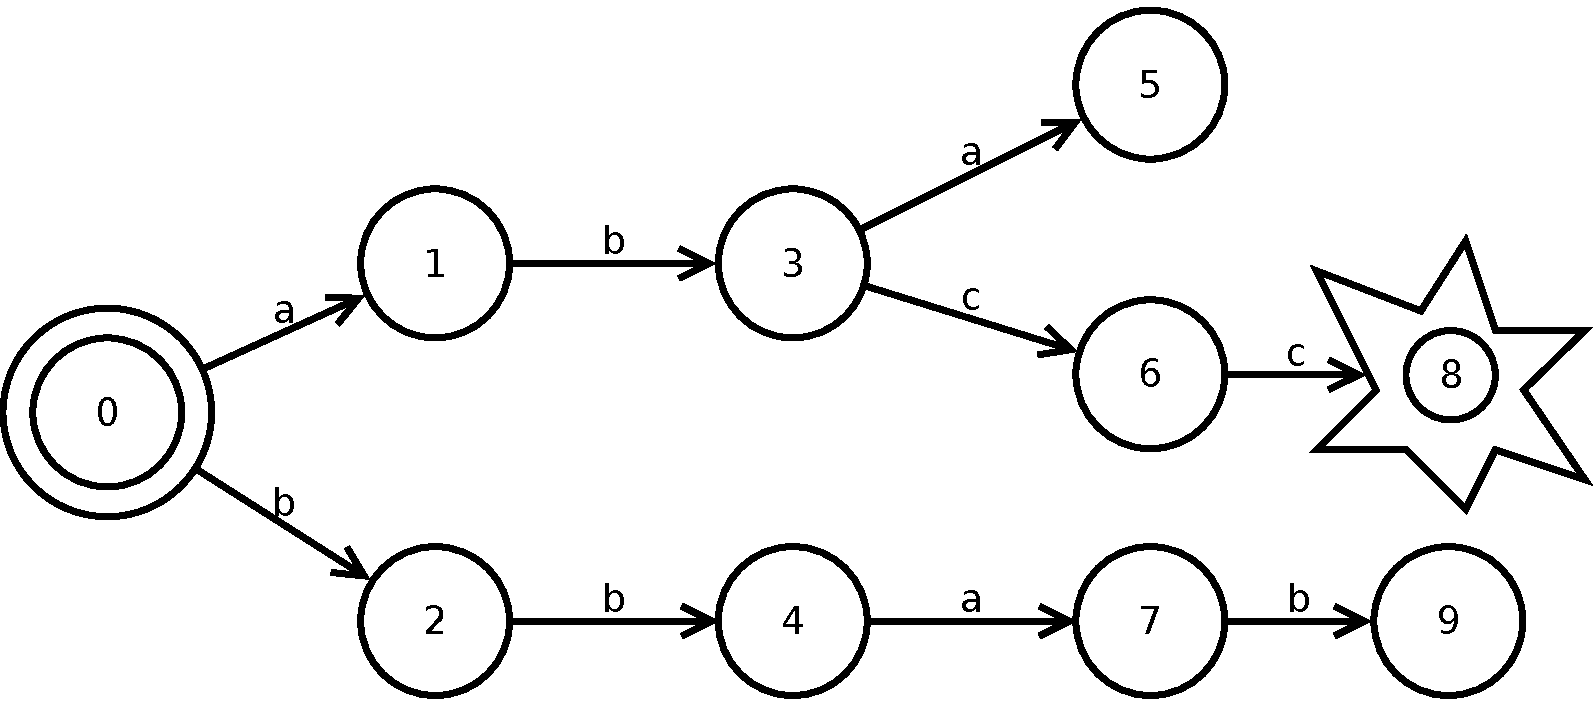
\includegraphics[width=8cm]{pictures/fsm1.pdf}
%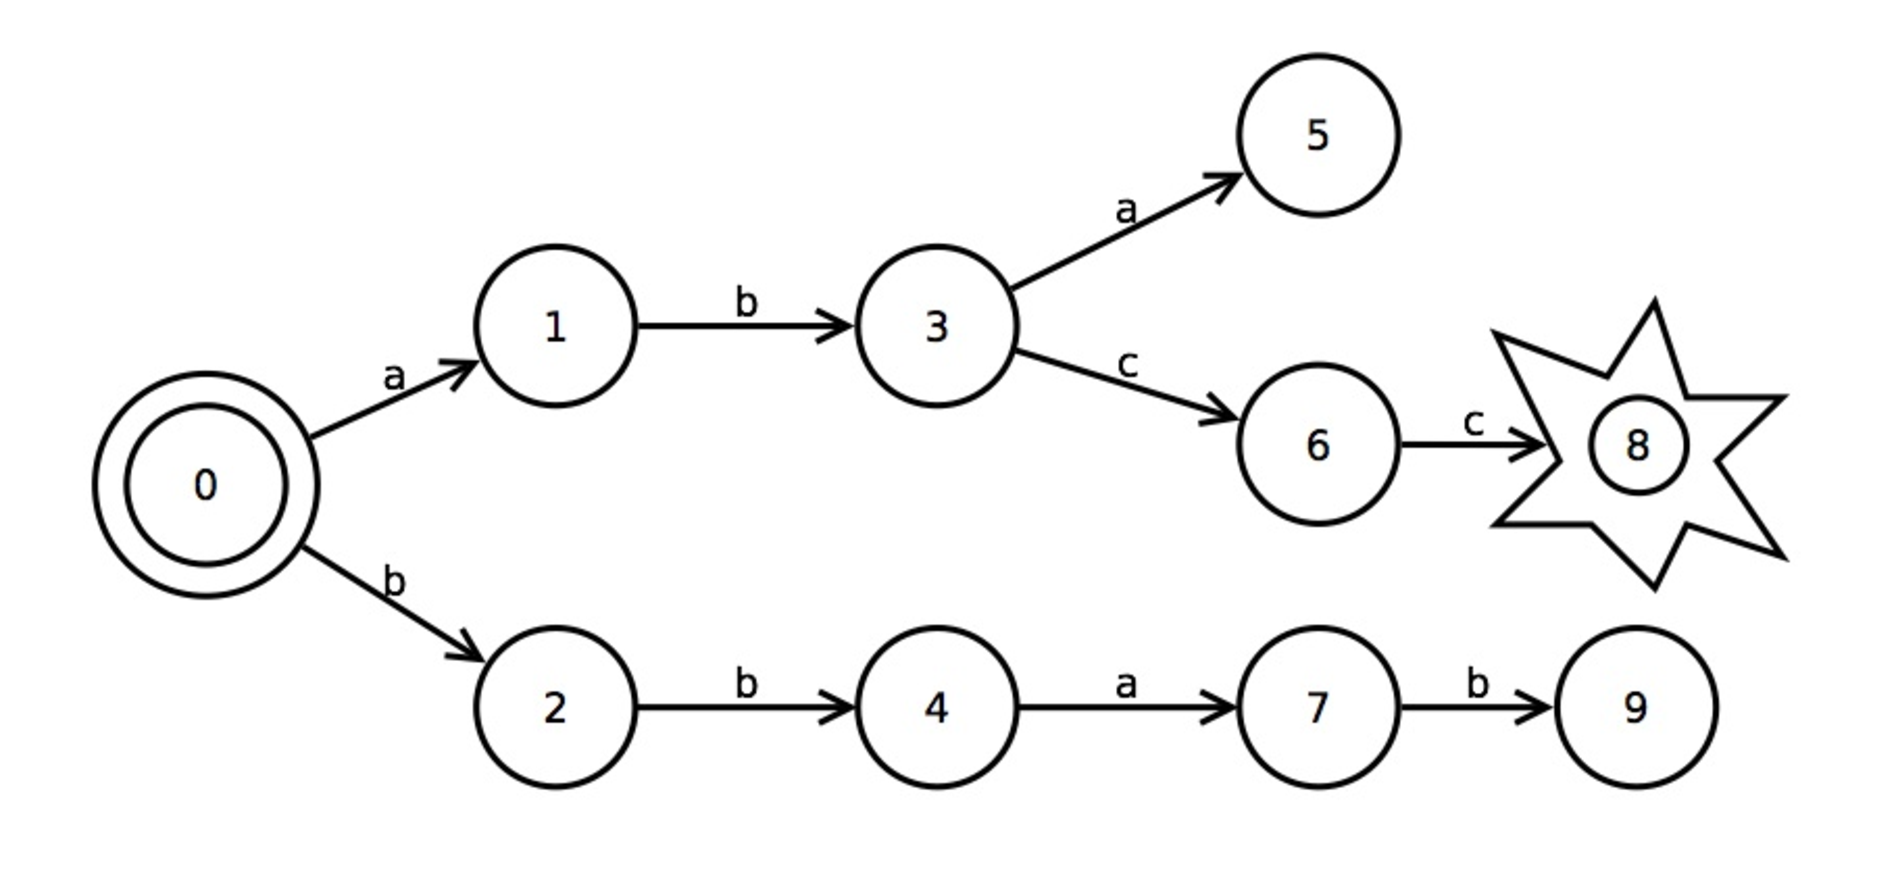
\includegraphics[width=8cm]{pictures/pic1.pdf}
%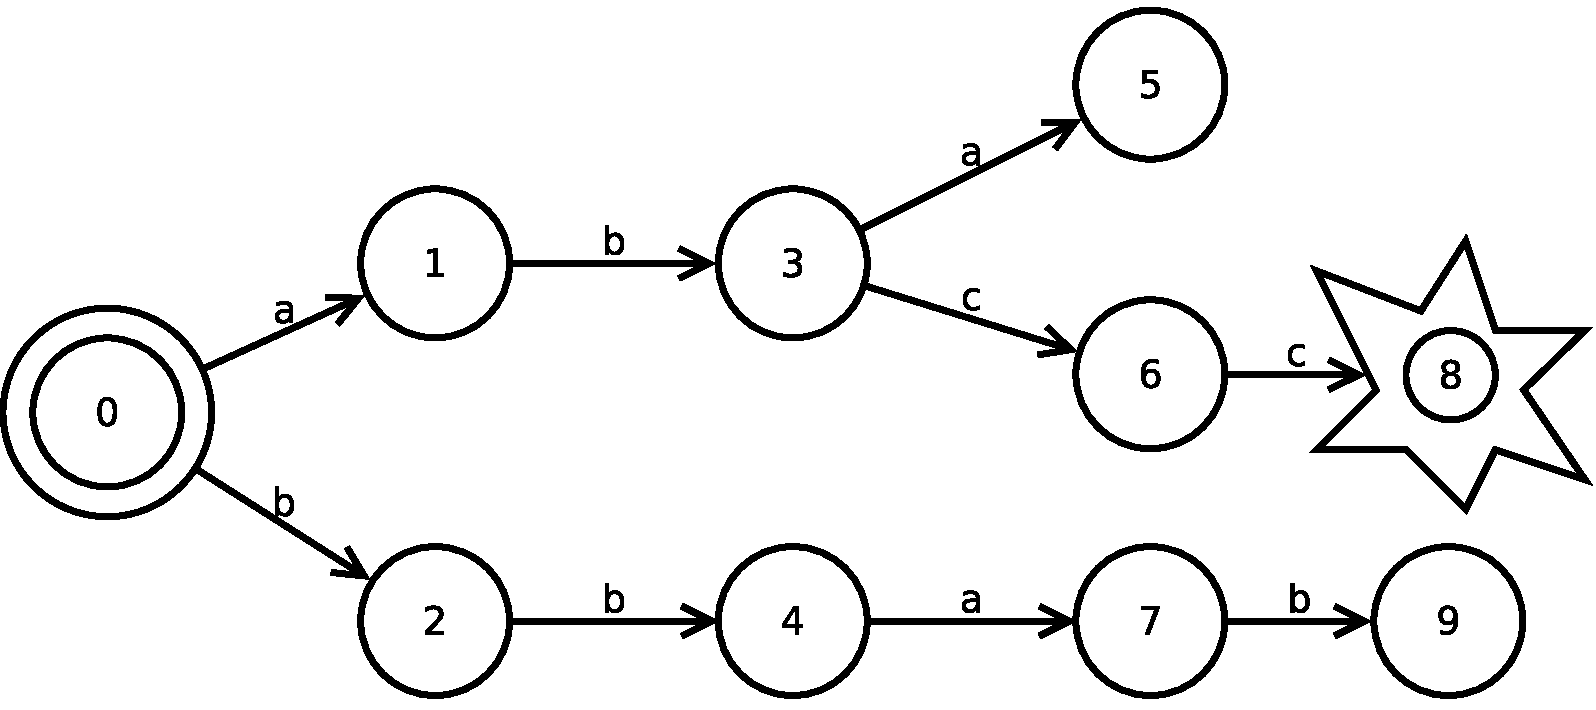
\includegraphics[width=8cm]{pictures/fsm1.ps}
\end{center}
\caption{Initial APTA}
\label{fsm1}
\end{figure}



\section{Erlang QSM}
\label{QSM}

We were unable to access the source code of the existing query-driven state merging (QSM) implementation, StateChum, but
we were able to consult two papers written by its developers
\cite{walkinshaw2008inferring,walkinshaw2007reverse}.
These papers describe how an implementation of
the QSM algorithm \cite{dupont2008qsm} is used to reverse engineer software.
We used the description in those three papers to re-implement the
algorithm in Erlang, and we describe that in this section. We were also able to use the original implementation to test our re-implementation, as we explain in  Section \ref{testing}.

The algorithm works in terms of regular languages, when using
it to reverse-engineer a program, we will consider traces
(execution sequences) as words in the language.
The QSM algorithm takes two sets of words, one set of words from
the language -- valid sequences of events -- and one of
words that do not belong to the language -- invalid sequences .
With one peculiarity, invalid sequences are invalid strictly
because of its last symbol, thus, if we remove the last event
from an invalid word, we should get a valid one. This corresponds to
an implementation raising an exception as last action in a trace.
There is no point in considering what happens after the exception
is thrown. From the input consisting in two sets of words, QSM will try to
produce the most general automaton that complies with the traces,
and this will hopefully give us an idea of the completeness of our tests.

In our implementation we take as event any Erlang term.
Nevertheless, for explaining the algorithm and for testing purposes,
we used atoms as events, thus, a trace corresponds to a list of atoms,
and the input to the algorithm is a tuple of two lists of lists of atoms,
(the positive ones first).

In this section we will use this set as example:
{%
\newcommand{\mc}[3]{\multicolumn{#1}{#2}{#3}}
\begin{center}
\begin{tabular}{ll}\hline
\mc{1}{|l|}{Positive} & \mc{1}{l|}{\texttt{[a,b,a]}}\\\cline{2-2}
\mc{1}{|l|}{} & \mc{1}{l|}{\texttt{[b,b,a,b]}}\\\hline
\mc{1}{|l|}{Negative} & \mc{1}{l|}{\texttt{[a,b,c,c]}}\\\hline
\end{tabular}
\end{center}
}%

\noindent
Which is represented by the Erlang term:
\begin{verbatim}
{[[a,b,a], [b,b,a,b]], [[a,b,c,c]]}
\end{verbatim}

The QSM algorithm roughly consists of two phases\cite{dupont2008qsm}. In the first one,
called \textit{initialization}, we create a finite state machine with a tree structure, the  Augmented Prefix Tree Acceptor (APTA)
that will accept all positive traces and reject all negative ones. In the
second phase, \textit{state merging}, we merge nodes of the tree in order to get
a smaller finite state machine which is still deterministic and accepts and rejects the initial sets of positive and negative traces. 

\subsection{Initialization}

The Augmented Prefix Tree Acceptor is the tree that we will use as
our initial FSM. It must necessarily have a tree shape, it must
accept all positive traces and reject all negative traces and
it must also be deterministic (this is, there cannot be two
branches with the same symbol departing from the same node).
For example, from the previous traces we would get the 
APTA in Figure \ref{fsm1} in which 0 is the initial state and 8 is a failing one.


In order to generate this in Erlang we create an initial
state with all the traces in it and extract the first event
from each trace. Then we create as many states as different
events we extracted and divide the rests of the traces
between the new states.

In the first iteration of our example we would get:

{%
\newcommand{\mc}[3]{\multicolumn{#1}{#2}{#3}}
\begin{center}
\begin{tabular}{lll}\hline
\mc{1}{|l|}{State} & \mc{1}{l|}{Kind of trace} & \mc{1}{l|}{New trace}\\\hline
\hline
\mc{1}{|l|}{1 (from a)} & \mc{1}{l|}{Positive} & \mc{1}{l|}{\texttt{[b, a]}}\\\cline{2-3}
\mc{1}{|l|}{} & \mc{1}{l|}{Negative} & \mc{1}{l|}{\texttt{[b, c, c]}}\\\hline
\hline
\mc{1}{|l|}{2 (from b)} & \mc{1}{l|}{Positive} & \mc{1}{l|}{\texttt{[b, a, b]}}\\\hline
\end{tabular}
\end{center}
}%

We repeat the process with every
new generated state until the states we generate do not
contain traces. When we arrive to the end of a positive trace
we just remove the trace, but when we fetch the last event of a
failing trace we generate a new failing state and check that there
are no traces left to expand from that state.

The target is to obtain the automaton as a record with the fields:
initial state, alphabet, states, transitions and failing states.
The transitions are stored using the labelled transition system (LTS),
as a list of tuples in the form: {origin, event, destination}. In
our example the transitions would look like:
\begin{verbatim}
[{0,a,1}, {0,b,2}, {1,b,3}, {2,b,4}, ..., {7,b,9}]
\end{verbatim}
We also decided to keep some order in the numbers of the states
to simplify the implementation of the \textit{state merging} later,
this way the number of a state in a given level would always
be smaller than the number of a state in a deeper level. This implied a
breadth-first processing which made the functions more complex
and added the need to keep a lot of information in the parameters.

This can be seen in one of the lowest level functions of the
\texttt{bluefringe\_apta} module: \texttt{expandTrace/2}.
The only purpose of this function
is to remove the first symbol from a trace and to add the related 
information to the automaton record.

We need to  remember the kind of the trace, positive or negative, 
the last state number granted,
the alphabet used (to add new symbols to it), the defined
rejection states, and a separate buffer with the already expanded
transitions from the current node, (in case our symbol already
has a transition).
To do this we wrote the function \texttt{breathfirst} that
updates the APTA recursively; as shown in  Figure \ref{breadthfirst}.
\begin{figure}
\begin{verbatim}
breathfirst(Apta, _State, [], _Map) ->
  Apta;
breathfirst(Apta, State, Traces, Map) ->
  {Accept, Ts1} = 
    lists:partition(fun(Trace) -> Trace==[pos] end, 
                    Traces),
  {Reject, Ts2} = 
    lists:partition(fun(Trace) -> Trace==[neg] end, 
                    Ts1),
  SameEs = 
    splitonhead(lists:usort([Map(E) || [E|_]<-Ts2]),
                Ts2,Map),
  {NextState,Transitions} =
    lists:foldl(fun({Hd,Tls},{NS,Trs}) ->
                    {NS+1,[{Hd,NS,Tls}|Trs]}
                end,{Apta#agd.lastSt,[]},SameEs),
  NewApta =
    Apta#agd{aSt = ifadd(Apta#agd.aSt,Accept,State),
             rSt = ifadd(Apta#agd.rSt,Reject,State),
             lastSt = NextState},
  lists:foldr(fun({Hd,NS,Tls},A) ->
                  NewA = [{State,Hd,NS}|A#agd.tr]
                  breathfirst(A#agd{tr = NewA},
                              NS, Tls, Map)
              end,NewApta,Transitions).
\end{verbatim}
\caption{The \texttt{breadthfirst} function}
\label{breadthfirst}
\end{figure}

\subsection{State merging}

Now we generalize the FSM by merging states. To merge two
states we just move the transitions from one state to the other.
For example, if we merge in the APTA above the states 1 and 2
we get the machine illustrated in Figure \ref{fsm2}.

\begin{figure}
\begin{center}
%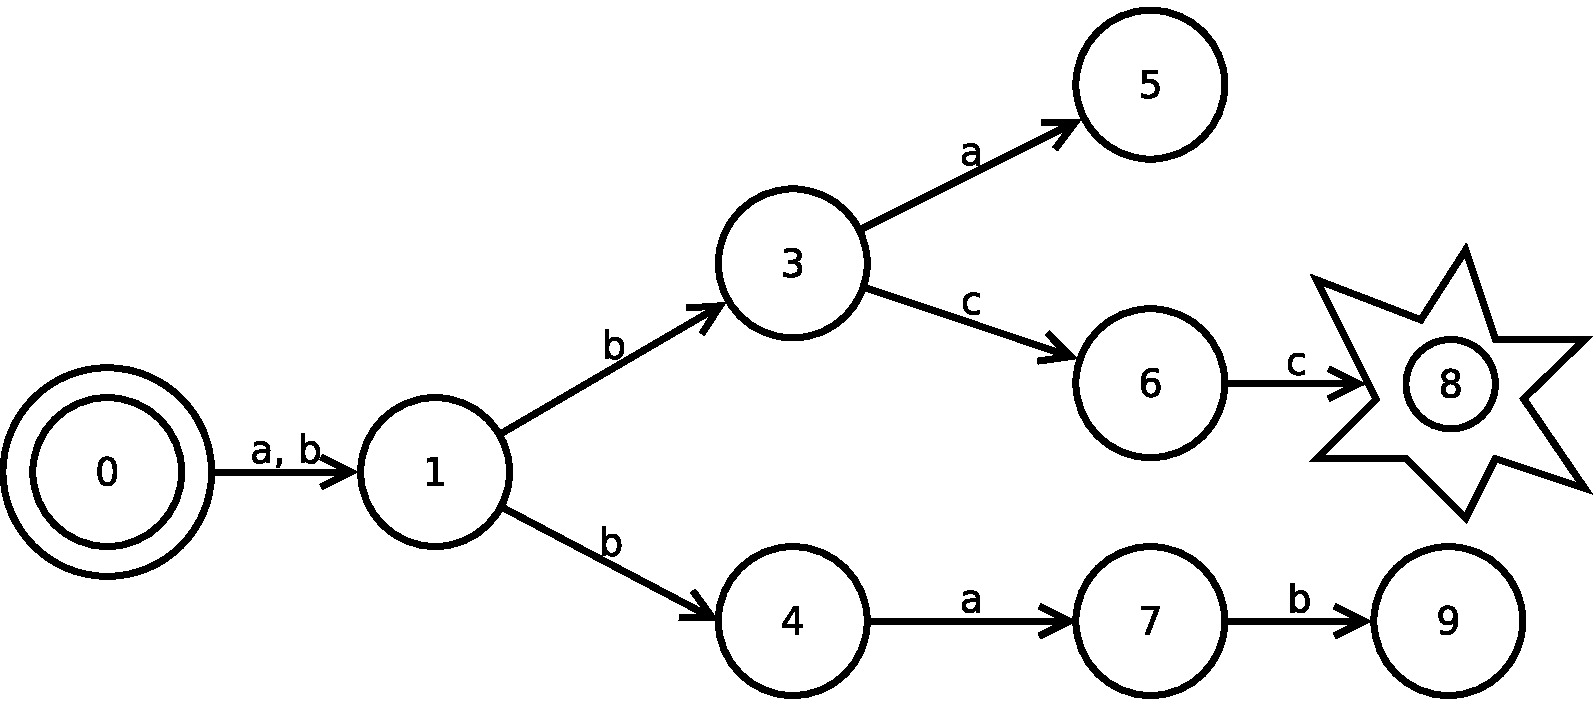
\includegraphics[width=8cm]{pictures/fsm2.ps}
%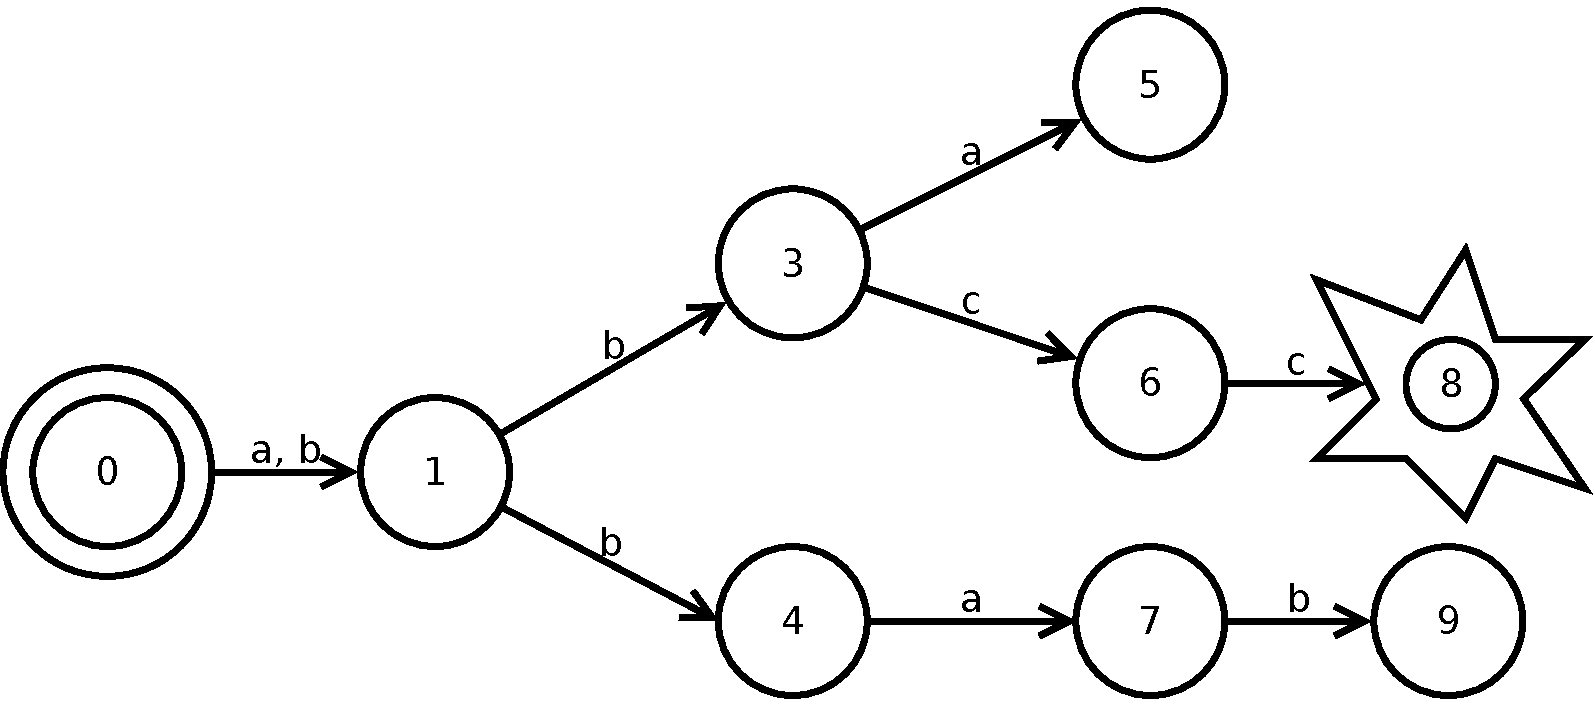
\includegraphics[width=8cm]{pictures/fsm2.pdf}
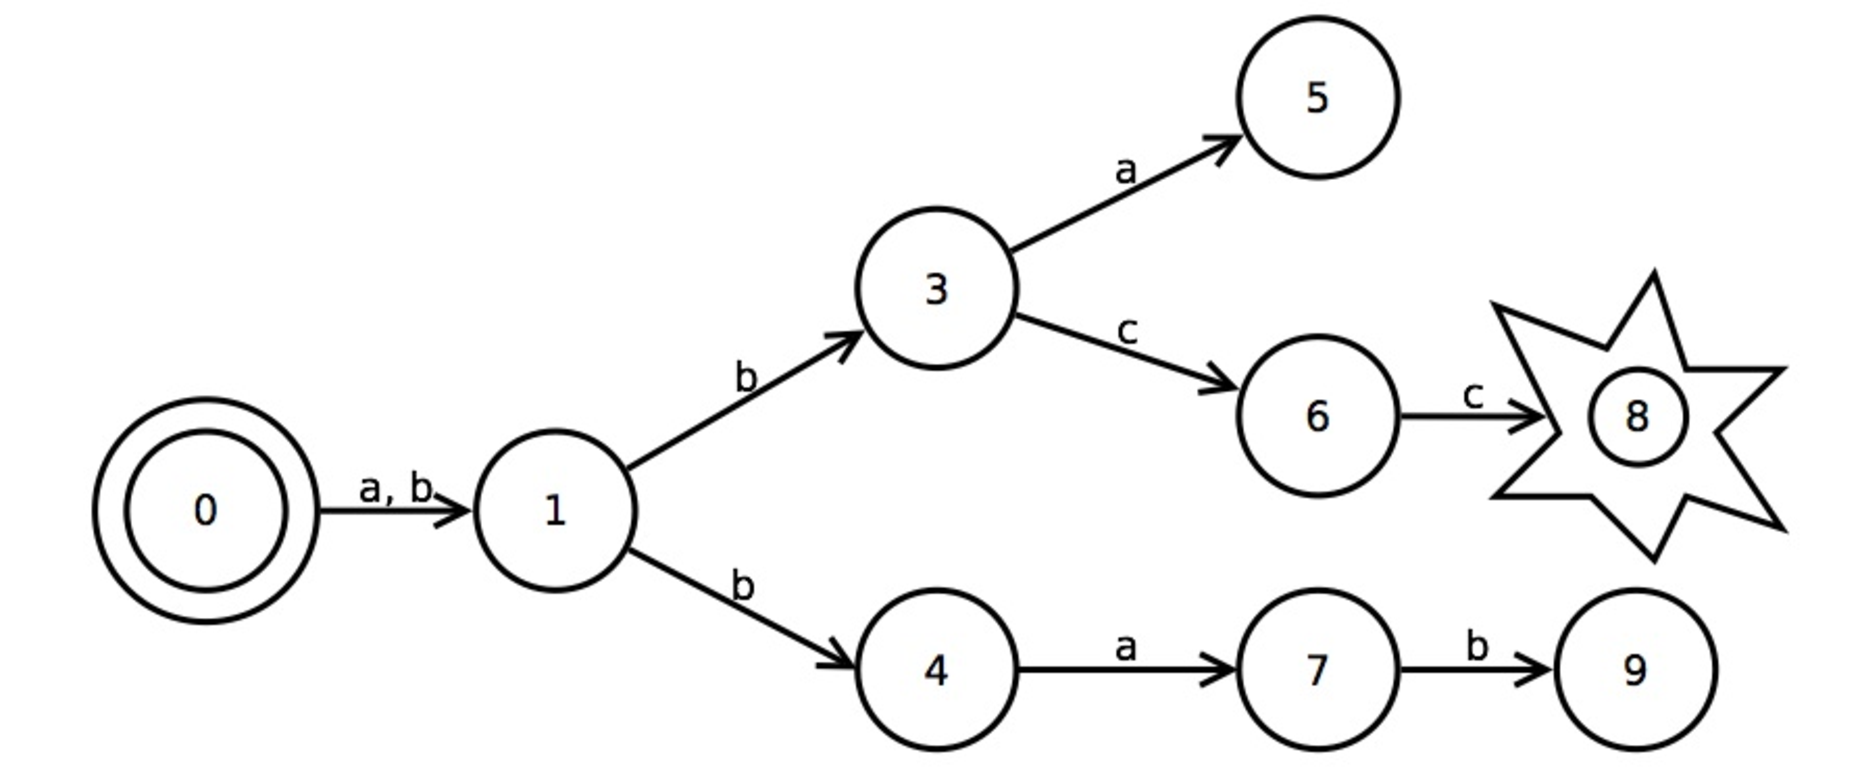
\includegraphics[width=8cm]{pictures/pic2.pdf}
\end{center}
\caption{State machine merging: stage 1}
\label{fsm2}
\end{figure}

If non-determinism appears we continue merging, 3 with 4, then
5 with 7 and we would get the machine illustrated in Figure \ref{fsm3}.

\begin{figure}
\begin{center}
%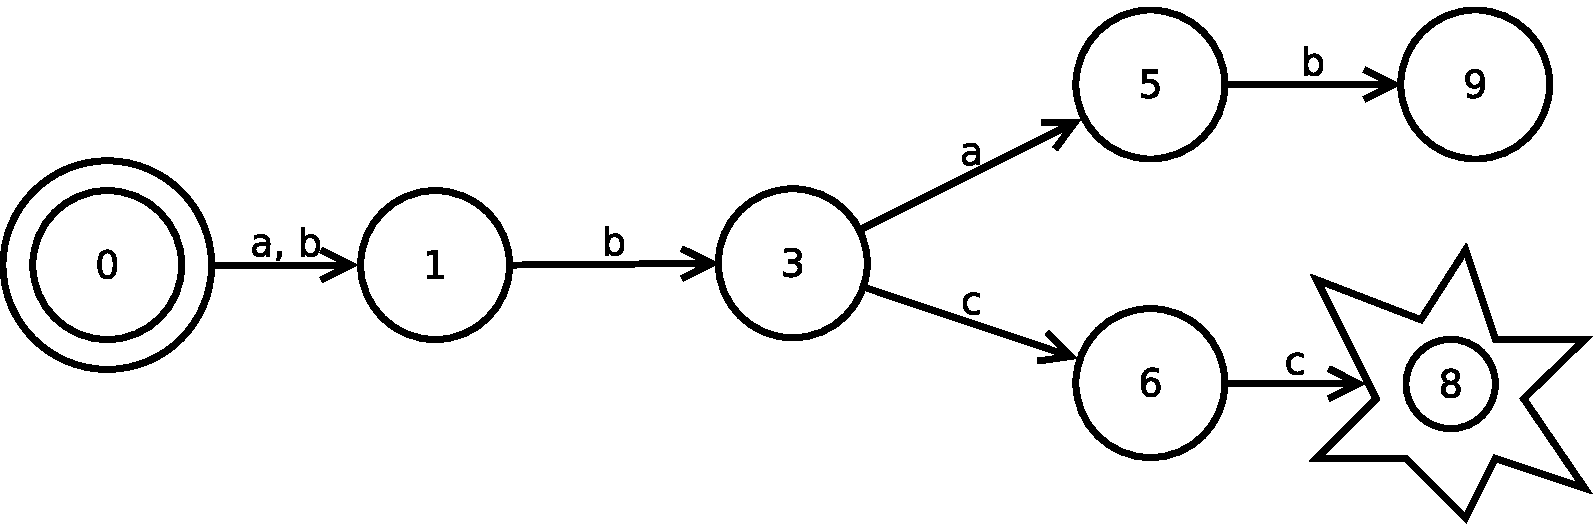
\includegraphics[width=8cm]{pictures/fsm3.ps}
%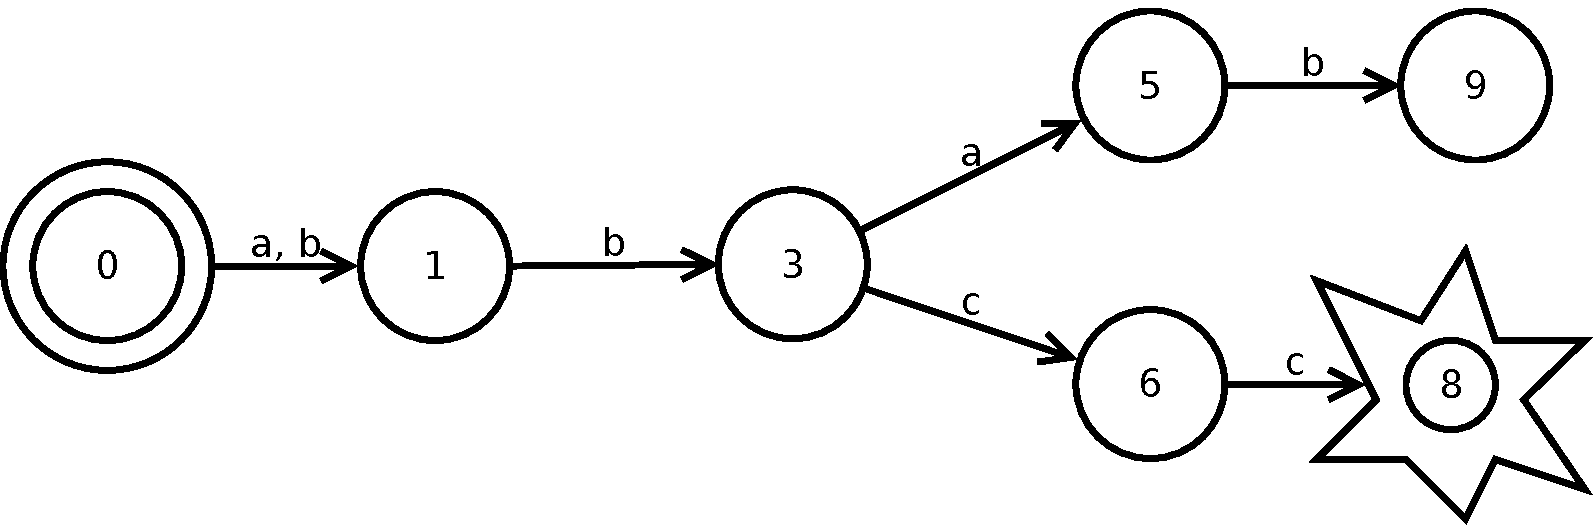
\includegraphics[width=8cm]{pictures/fsm3.pdf}
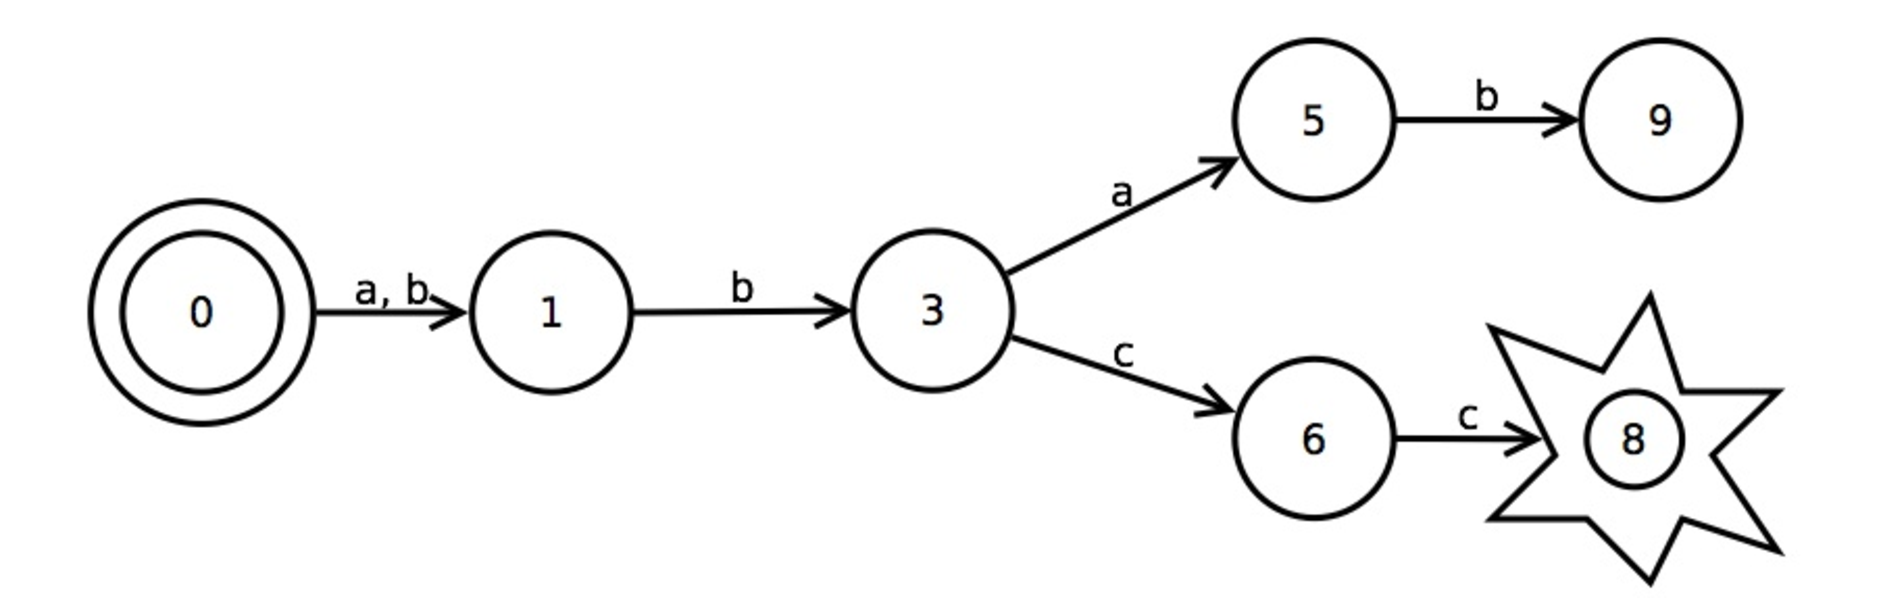
\includegraphics[width=8cm]{pictures/pic3.pdf}
\end{center}
\caption{State machine merging: stage 2}
\label{fsm3}
\end{figure}

After merging, we check that the original traces are still
valid. If any trace is lost we undo the merge. In our implementation
this is done by throwing an exception which interrupts the merging
when this happens.

To decide which nodes should be merged first we use the \emph{
blue-fringe} strategy. This strategy consists in considering two zones of the
FSM. The red zone has the nodes that cannot be reduced
and the blue zone has the immediate neighbours, which will
be used as candidates to merge with the red zone.

\begin{figure}
\begin{center}
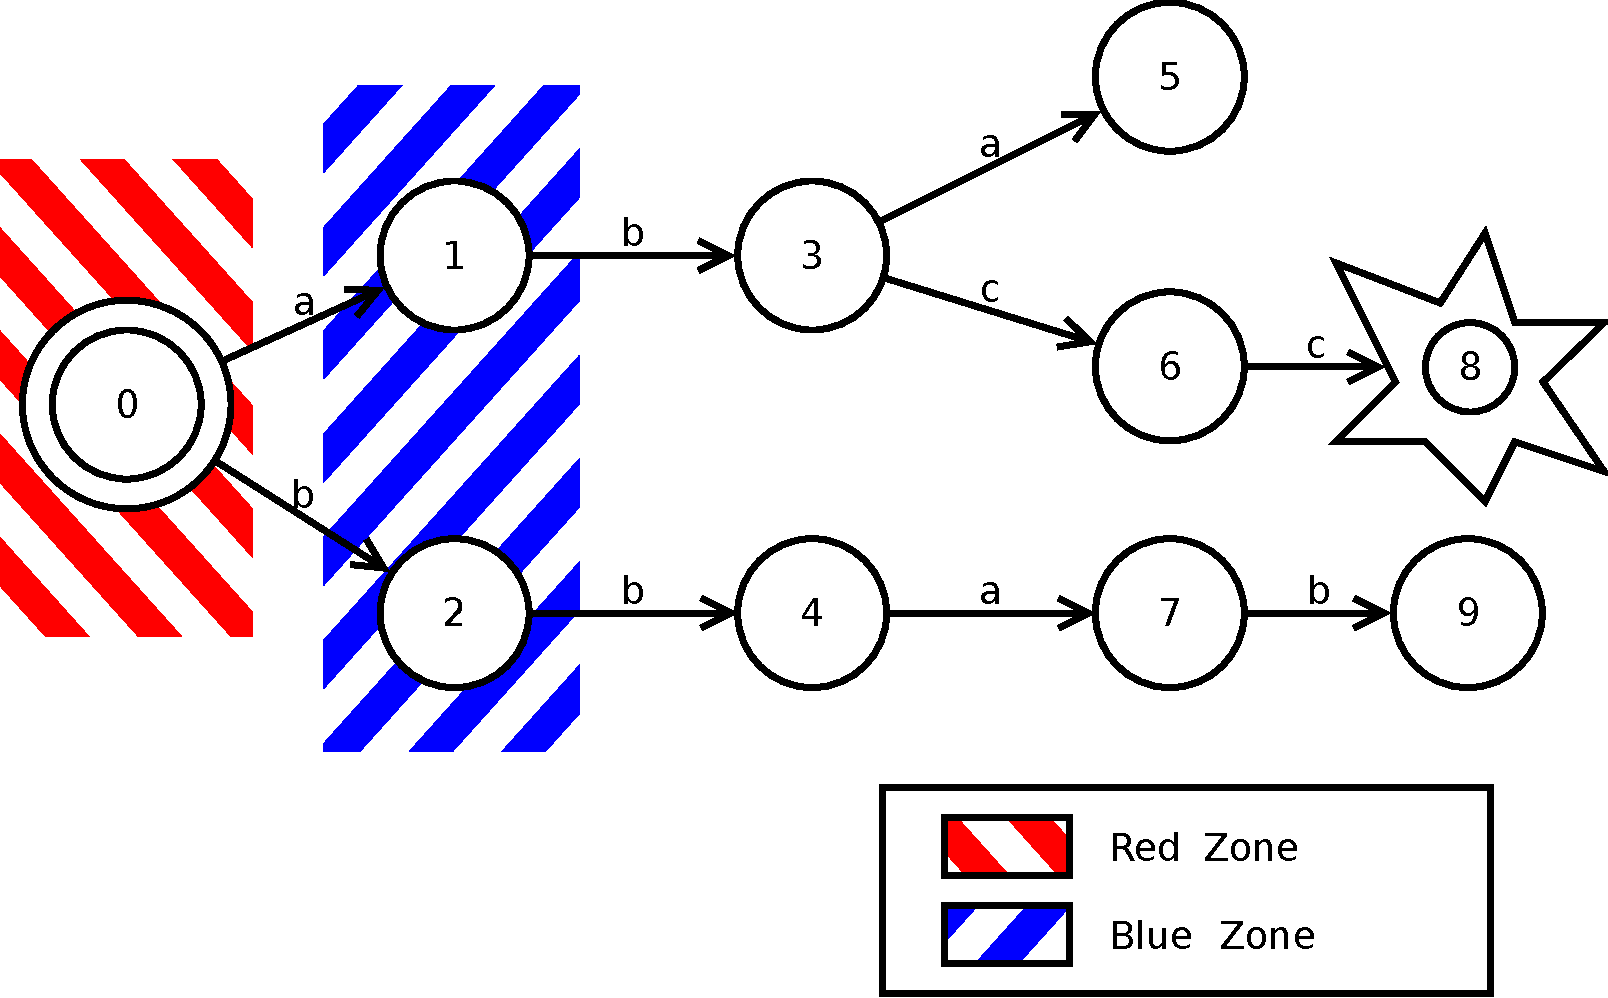
\includegraphics[width=8cm]{pictures/fsm4.pdf}
%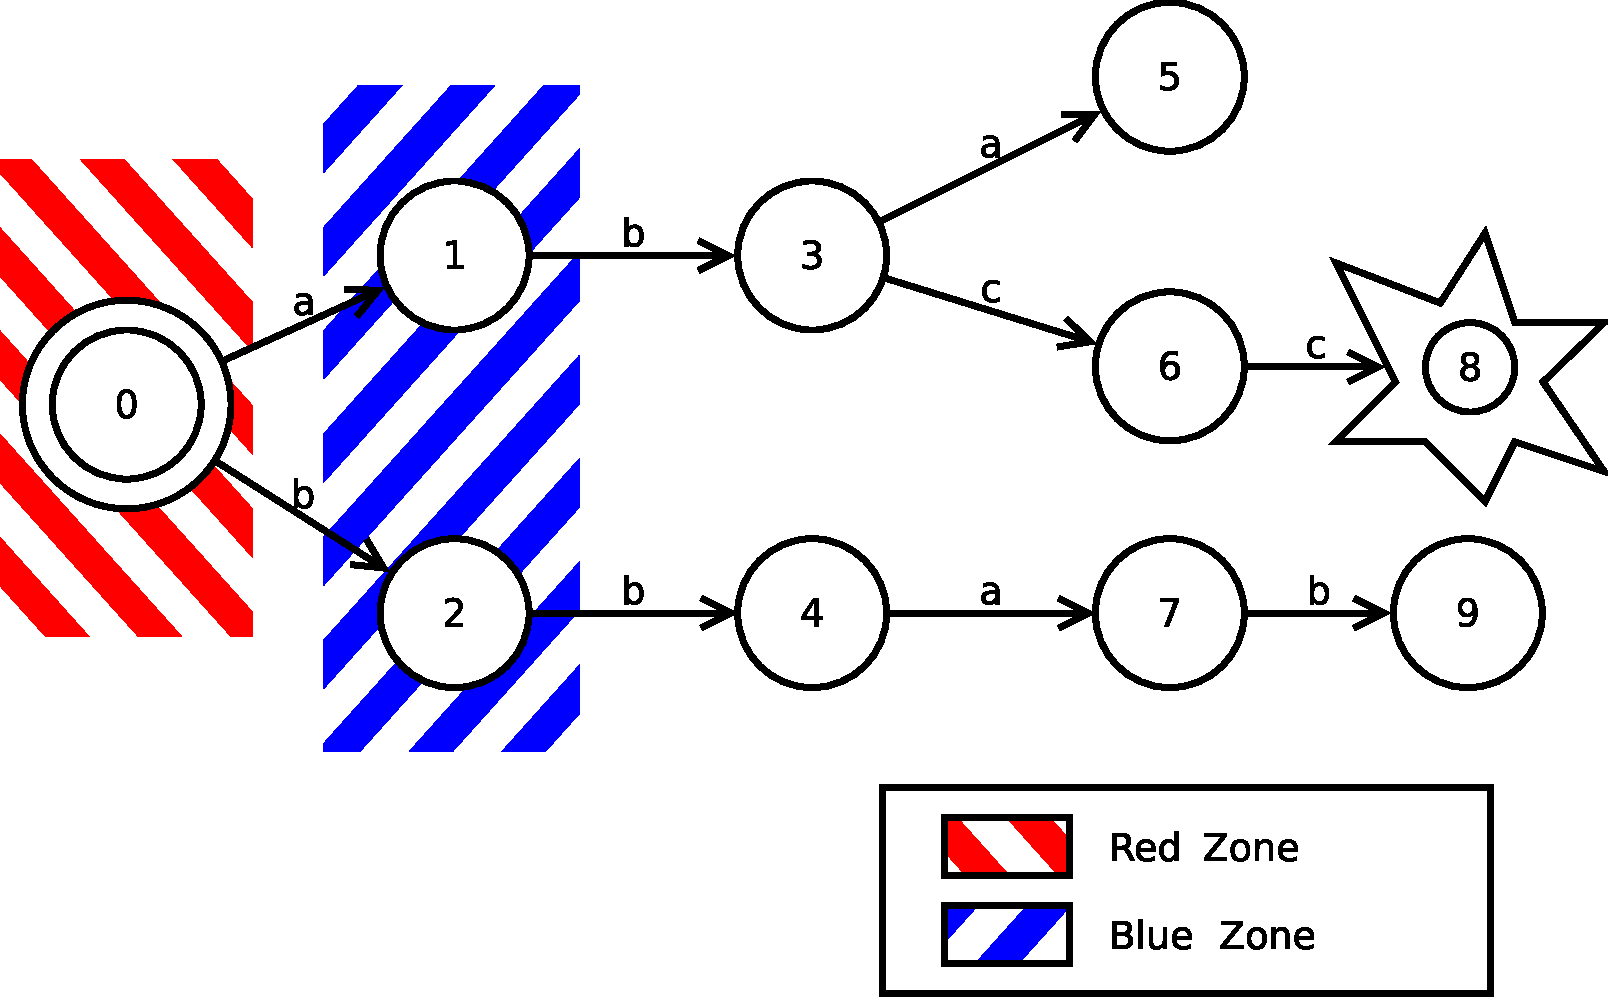
\includegraphics[width=8cm]{pictures/fsm4.ps}
%\includegraphics[width=8.5cm]{pictures/pic4.pdf}
\end{center}
\caption{State machine merging: stage 3}
\label{fsm4}
\end{figure}


We start setting the initial state as red and its neighbours as blue.
At each step we compute the score for every possible pair of candidates
to merge, (pairs consisting on one node from the red zone and one node from the blue zone).
The score for a pair of candidates is given by the number of extra
merges that we would be forced to carry out in order to restore determinism after
hypothetically merging that pair itself.

\begin{center}
\begin{tabular}{c||c|c}
Pair & (0, 1) & (0, 2)\\\hline\hline
Score & 1 & 3
\end{tabular}
\end{center}

Two states are incompatible if one of them is a failing state, and
the other is not. If a pair of candidates is incompatible or if
it forces us to make an incompatible merge (in order to restore determinism)
its score will be $-1$.

We must also check that all the positive traces are accepted and
all the negative traces are rejected before actually committing
any merge.

If a blue node cannot be merged with any of the red nodes,
it becomes red and the blue zone is updated accordingly to
match all the immediate neighbours of the new red zone.

The process ends when the whole FSM is red and we wrap up by
merging all the failing states in one. This last merging should
not produce indeterminism since there should not be transitions
starting in any failing state.

\subsection{Additional considerations}

QSM was initially designed to be interactive, here we only
focus in the non-interactive version. The main difference is that the interactive
version is intended to generate sample traces during the merging process and to ask
the user if those are valid, in order to avoid over-generalization.
Nevertheless, the same results can be achieved with the passive
implementation. The user only has to add new tests to the input
and to run the algorithm again, and this is supported by the integration described in Section \ref{improving}. Alternatively
the algorithm could learn from running additional tests, but this is not implemented at present. 

Having the QSM algorithm implemented in Erlang
gives us a better integration with the test code than would be possible with other languages, (e.g.\ Java, in the case of StateChum), since for
example it allows us to use arbitrary Erlang terms as traces, which allows fine control of the abstraction mechanism in model formation as explained below.

After finishing the implementation, we also noticed that it executes
faster than the original StateChum, since it does not need to start an extra virtual machine for this sole purpose.

\section{Testing}
\label{testing}

In order to verify correctness of our new implementation
we have used QuickCheck to test it against StateChum \cite{statechum}
because we wanted it to have the same behaviour as this already well-tested
implementation.

We test that, for a given set of positive and negative traces,
our implementation and StateChum give similar state machines.
In other words, we use StateChum as an oracle for our model based testing.

\subsection{QuickCheck testing}

To test our implementation of QSM we first used a property
that should hold after the execution of the algorithm. The positive
traces that were provided as input must be accepted by the output
automaton. And the negative traces must be rejected exactly at their
last symbol, this is, they must drive us precisely from the initial
state to a failing one.

Implementing just this property in QuickCheck would be simple if we only
generated completely random sets of traces. But, if we do it that way,
most of the generated sets of traces that we would get would lead to
meaningless automata that would have nothing to do with the ones we
would find in a real scenario. To solve this issue we decided to
generate random automata instead, and then walk through them randomly.
This implementation could result in unreachable states, but this is not
a problem since the input to the algorithms is just the trace sets and they
will not contain any such states.

An automaton in the testing module is represented by a tuple of the form:
\begin{verbatim}
{list of states, 
 initial state (init), 
 failing state (bad), 
 list of events, 
 list of transitions}
\end{verbatim}
and each
transition is as usual another tuple:
\begin{verbatim}
{Origin, Event, Destination}
\end{verbatim}
and QuickCheck generators for automata and transitions are given in Figure \ref{generateAT}.

\begin{figure}
\begin{verbatim}
automata() ->
  ?LET({States,Events}, 
             {set(elements([a,b,c,d,e,f,g])),
              non_empty(set(elements([x,w,y,z])))},
     ?LET(Trs, transitions(Events,States),
     {[init,bad] ++ States,init,bad,Events,Trs})).

transitions(Events, States) ->
  ExtStates = [bad|States],
  ?LET(Trs, 
        [{init,elements(Events),oneof(ExtStates)}|
	         normal_transitions([init|States], Events, 
	                             [init|ExtStates])],
	 determinize(Trs)).
\end{verbatim}
\caption{Generators for automata and transitions}
\label{generateAT}
\end{figure}

In the \texttt{transitions/2} function we make sure that we get at least one transition
so that later we can generate at least one trace.

In order to make valid and useful automata we  have to treat the
initial state (\texttt{init}) and the failing state (\texttt{bad})
separately and to make sure that we do not generate transitions
that start in the failing state.

Note that these generators can cause a trace to be both positive and negative, leading to inconsistency. This corresponds to a negative test, since both StateChum and our implementation should reject such examples. As long as this happens infrequently, which it does, the few negative tests take little effort from the total testing time.

After generating a random automaton, we just do a series of
random walks through the automaton (starting at the initial state),
give them as input to the algorithm, and check that the output automaton
complies with the input traces.

This helped us to find some misunderstandings in the implementation. For
example: we thought at first  that just by taking care of not
merging a normal state and a failing one, the collapsed automaton would
properly accept or reject all the input traces, but this was proved to
be false when we ran this test. We fixed it by checking the traces with
each merge. But even though these tests were useful, it would still pass
if we had only implemented the APTA generation, and consequently we are
not actually testing that the merging mechanism and the blue-fringe
implementation work properly.

\subsection{Interfacing StateChum}

Specifically, we wanted to know if our implementation generated minimal
automata. We could not find an alternative way to check if the resulting
automaton was in fact minimal, since that is the actual purpose of the
QSM algorithm.
But we did know StateChum, an already tested implementation, that does give
a minimal automaton. So we checked instead that our implementation gave similar
results. In order to do this, we first wrote an interface to StateChum
that would allow us to provide lists of atoms as input, and then parse the
resulting automaton to an Erlang entity. This could be done thanks to the
text mode of StateChum.

By exporting StateChum's automaton in text format, we can parse it and
compare it to our own automaton. However, StateChum's output does not specify
the initial state or transitions that end in a failing state, or the failing
state at all. Because of this, we first only compared the number of 
non-failing states.

Already this simple check allowed us to realize a misunderstanding
of the semantics of the algorithm. For example: blue states need to
be transformed to red immediately after they become impossible to merge
with the red ones, instead of trying to merge all possible blue states
first.

Another example is that in the original pseudo-code there are
instructions of the kind \texttt{for all X} where the list \texttt{X}
grows while execution is inside the loop. After testing we
discovered that these changes should be taken into account by
performing extra iterations at the end.

\begin{figure}
\begin{center}
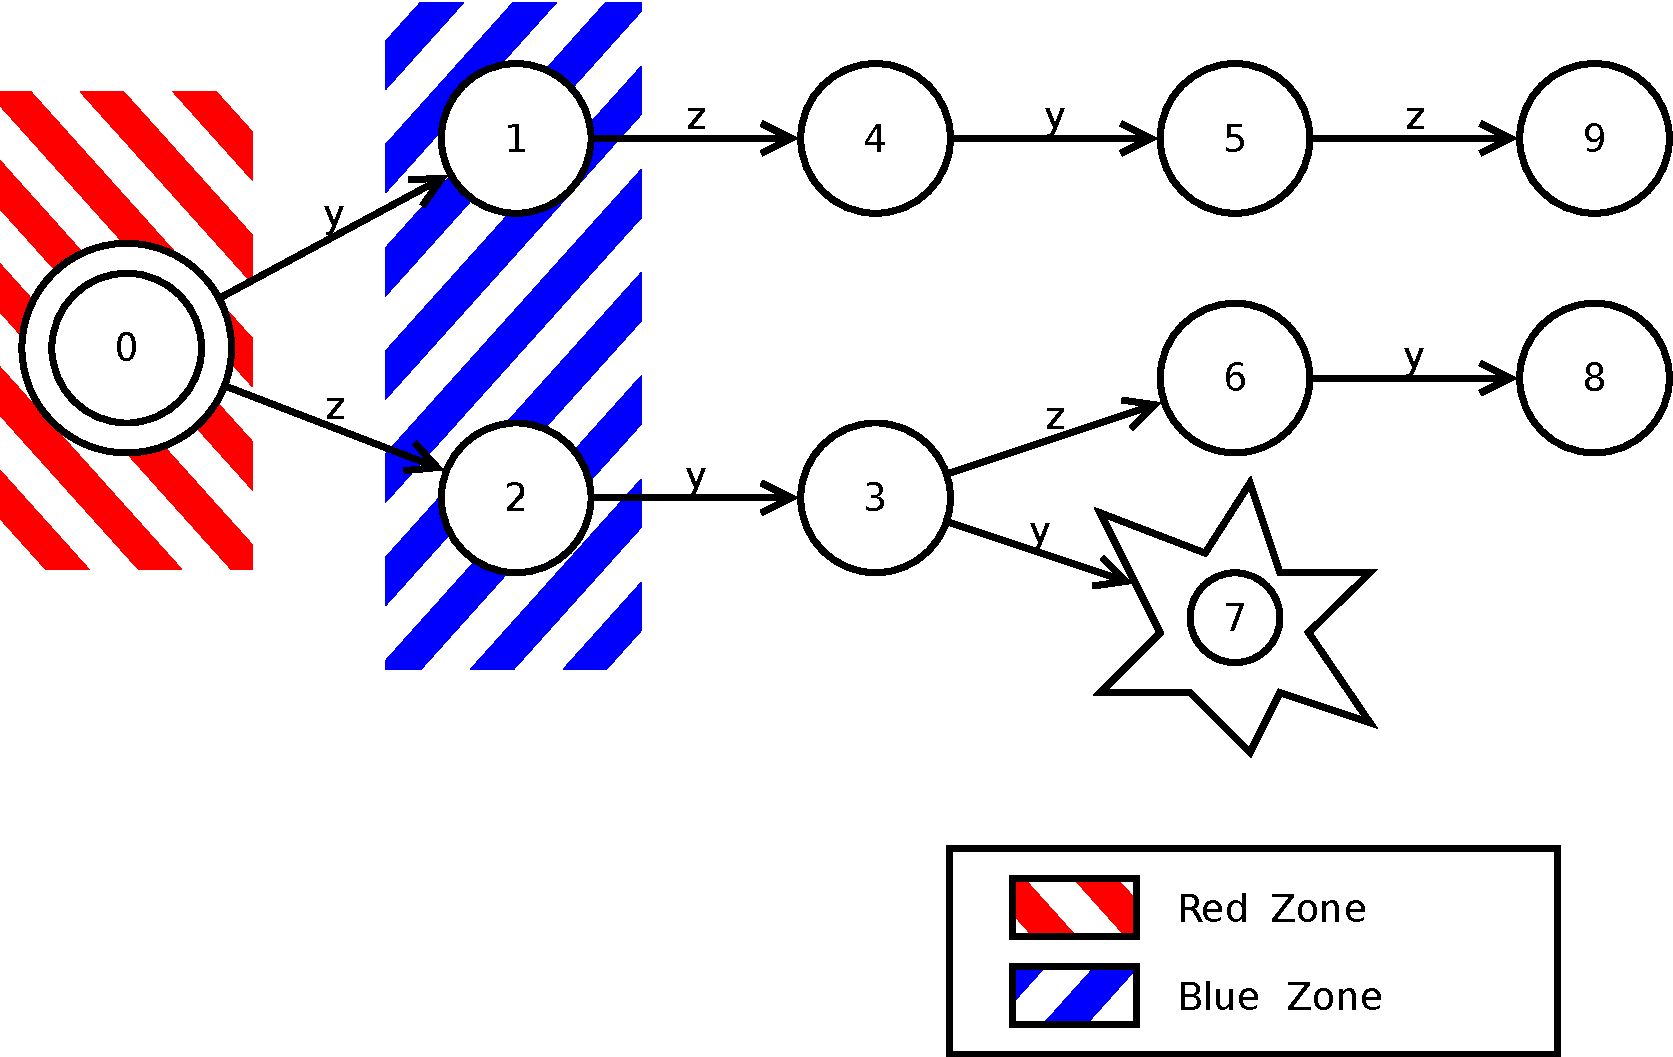
\includegraphics[width=8.5cm]{pictures/fsm5.pdf}
%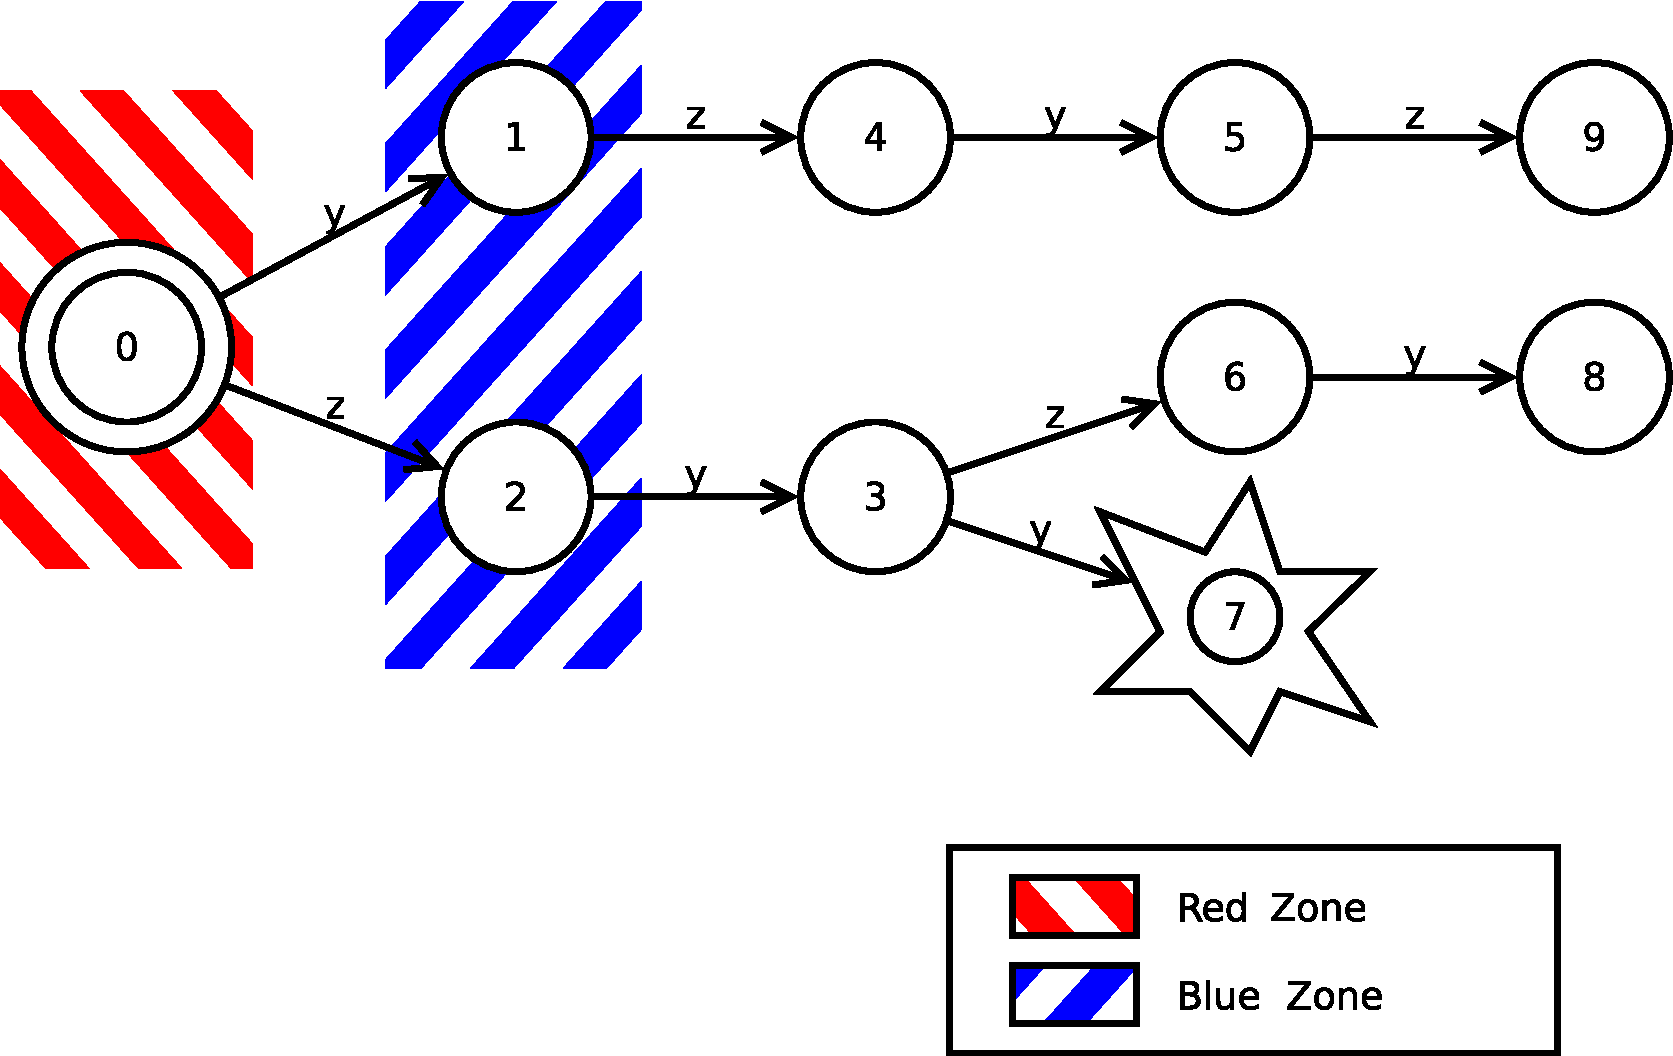
\includegraphics[width=8.5cm]{pictures/fsm5.ps}
%\includegraphics[width=8.5cm]{pictures/pic5.pdf}
\end{center}
\caption{Alternative APTA}
\label{fsm5}
\end{figure}

\subsection{Differences from StateChum}

We needed to fix a few errors in our QSM implementation, but even after that,
we found out that in some cases the results were still different despite
being both correct according to the QSM specification.
For example, the traces 
\begin{verbatim}
{[[y,z,y,z],[z,y,z,y]],[[z,y,y]]}
\end{verbatim}
result in the APTA tree shown in Figure \ref{fsm5}.
Then we apply the bluefringe strategy and compute the scores for all possible
combinations:

\begin{center}
\begin{tabular}{c||c|c}
Pair & (0, 1) & (0, 2)\\\hline\hline
Score & 3 & 3
\end{tabular}
\end{center}
One obvious question arises: If several pairs of nodes have the same score,
which pair shall we merge first?

If we choose the pair (0, 1), (as StateChum apparently does in this case), we will
form a loop with the \texttt{y} symbol transitioning to state 0 and continuing with
the algorithm we will end up with an irreducible automaton shown in Figure \ref{fsm6}, where state 
numbers may differ.

\begin{figure}
\begin{center}
%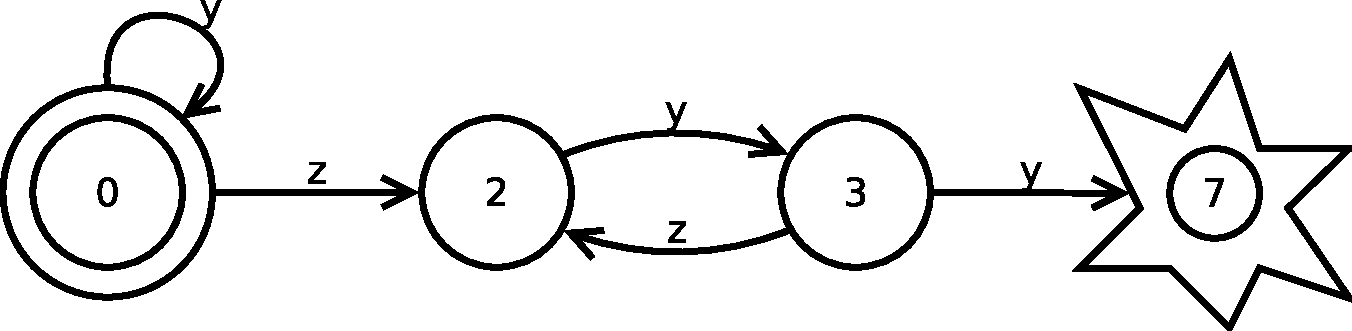
\includegraphics[width=8cm]{pictures/fsm6.ps}
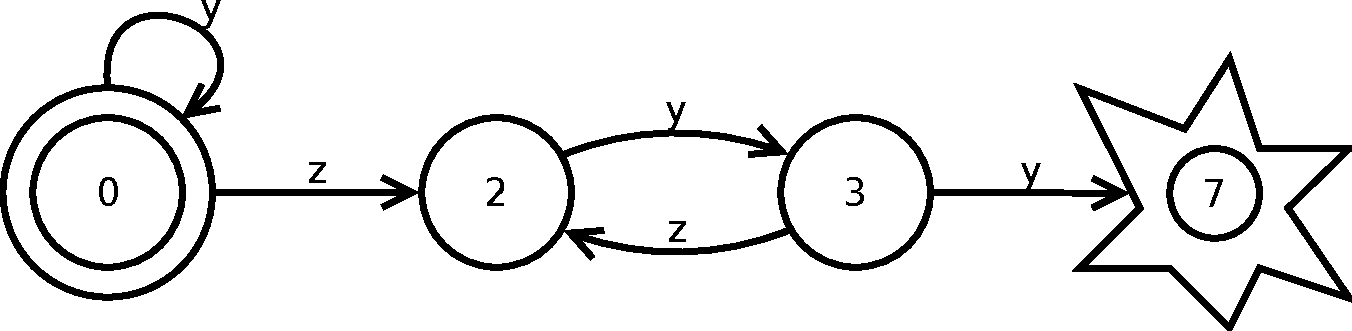
\includegraphics[width=8cm]{pictures/fsm6.pdf}
%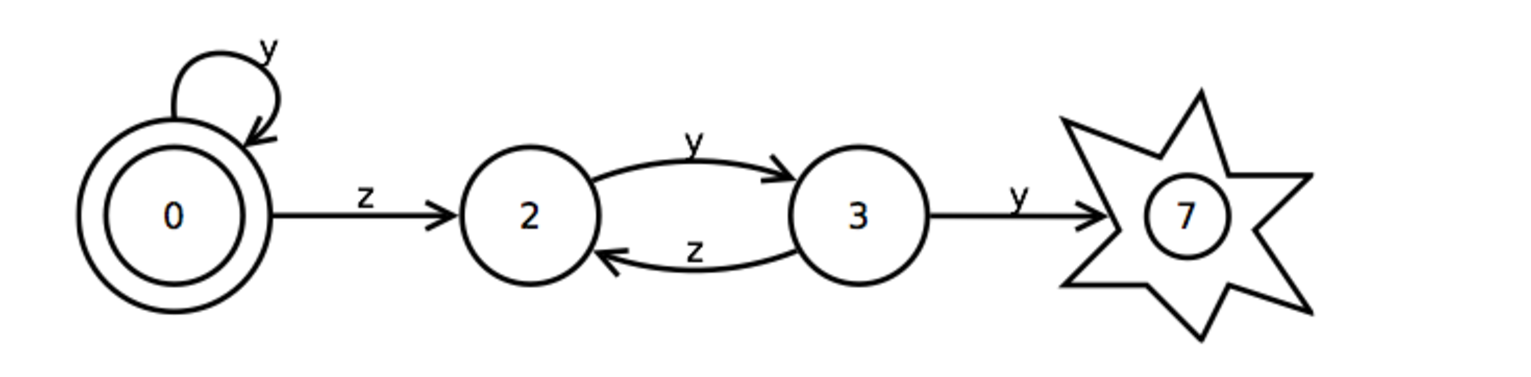
\includegraphics[width=8cm]{pictures/pic6.pdf}
\end{center}
\caption{Irreducible automaton version 1}
\label{fsm6}
\end{figure}
 
On the other hand, if we chose the pair (0, 2), (as our implementation does in this
case), we will form a loop with the \texttt{z} symbol transitioning to state 0 and
we will get a slightly smaller, also irreducible automaton, shown in Figure \ref{fsm7}.

\begin{figure}
\begin{center}
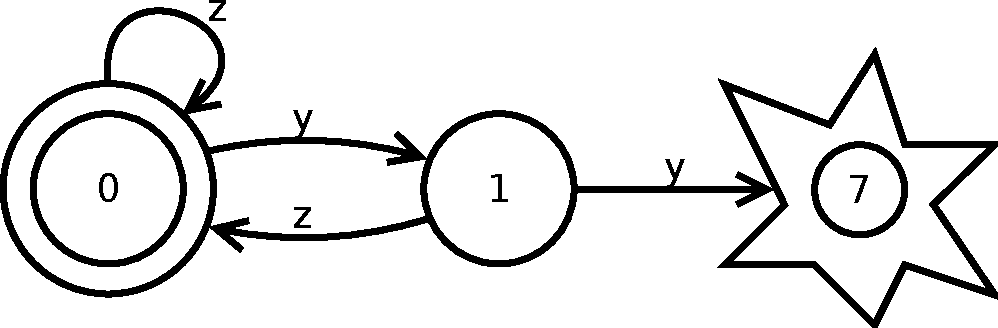
\includegraphics[width=6cm]{pictures/fsm7.pdf}
%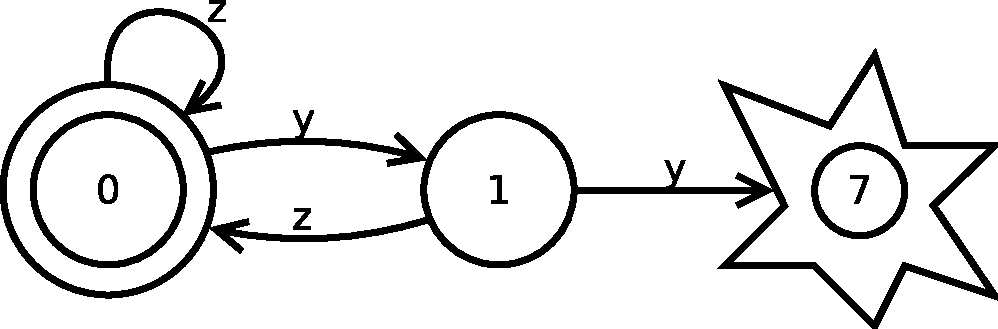
\includegraphics[width=6cm]{pictures/fsm7.ps}
%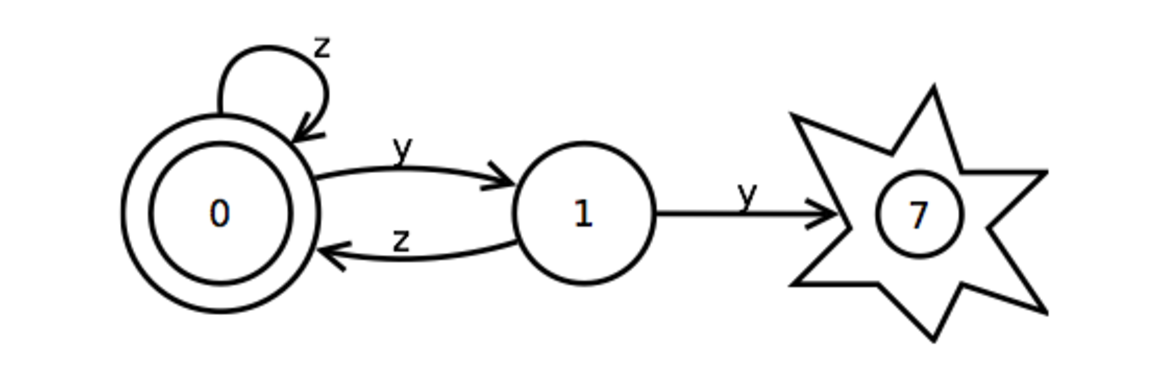
\includegraphics[width=6cm]{pictures/pic7.pdf}
\end{center}
\caption{Irreducible automaton version 2}
\label{fsm7}
\end{figure}

Given this choice in implementation, the question arises whether any of the
choices is better than the other? In order to find out, we used QuickCheck again. 
We generated a large number of inputs
and tested the two algorithms on these inputs and compared the size of
the resulting automata. With the QuickCheck \texttt{collect()} function we
collected statistics on how
many times our implementation produces similar results, how many times StateChum
produces a smaller example, and, how many
times our implementation results in a smaller automaton. The result for 1000
iterations was:

\begin{verbatim}
OK, passed 1000 tests
89% draw
5% sc
5% qsm
true
\end{verbatim}
where \texttt{sc} indicated that the output from StateChum was smaller, \texttt{qsm}
that the output from our tool was smaller and \texttt{draw} that both
outputs had the same size.

From this we can conclude that, despite the fact that the decision does affect the size of
the resulting automaton, our choice
outputs approximately the same number of automata bigger and smaller than
StateChum and, approximately ninety percent of the time both implementations result
in automata of the same size.


\section{From EUnit tests to traces}
\label{EunitToTraces}

EUnit \cite{eunit,eunit_user_guide} is the Erlang unit test framework in the
style of JUnit, CUnit, etc. In this framework one can specify unit tests
and check that their results are correct by using some preprocessor macros
provided by the EUnit library. By using this tool we can later run all
the unit tests at once and get a summary of those results.

EUnit modules contain a series of functions that can in principle
contain any Erlang expression, these expressions are
evaluated when the tests are run. Because of this, the tests
can have arbitrarily complex structures, which makes it difficult, (and
in some cases impossible) to analyse them statically. We could instead
trace calls to the subject under test. But this is not always possible since we may not have
the implementation, and thus, the tests may not be possible to execute.
In fact, when we follow test driven development, some of the tests are always ahead
of the implementation and need be statically analysed instead of traced.
Thus, depending on the use case for our tool, we would
like to have both static analysis as well as dynamic analysis and combinations
thereof. 

\subsection{Possible scenarios}

From the syntactic point of view, the tests in EUnit are given by
normal Erlang functions with a name that ends with the suffix \texttt{test}
or \texttt{test\_}. They are also expected to contain calls to some of the EUnit macros
like \texttt{?assertMatch()} or \texttt{?assertException()} which are
defined in the header file \texttt{eunit/include/eunit.hrl} from the
EUnit distribution.

Execution flow may vary in terms of the returned values
from other functions. These other functions may be auxiliary test functions or they may indeed be in the target code that we want to test,
and so they may not yet even be
defined.

On the other hand, in some cases we may find that all the external
functions are surrounded by macros like \texttt{?assertMatch()} or
\texttt{?assertException}, and in those cases we would know the
expected return value.
This gives us three possibilities to obtain traces of tests:
\begin{enumerate}
 \item Dynamically running all tests and collecting the traces. We describe our approach to this in Section \ref{dynamic-collection}.
 \item Dynamically running the part of the tests that is in the same
module and inferring the return values from the EUnit macros when
possible.
 \item Statically parsing the EUnit code and trying to infer the
execution flow when possible.
\end{enumerate}
None of the three would work for all possible cases, but
 we chose to implement the first and the last one to show the different approaches that can be used, the former to give maximum fidelity to the implementation and the latter to achieve the maximum independence from the tested code. Section \ref{static} covers static extraction and Section \ref{dynamic-collection} covers dynamic trace collection.

\section{Static trace extraction from EUnit}
\label{static}

EUnit can be considered to be a domain specific language for testing. Common Erlang test patterns are encapsulated in a comprehensive set of macros. We do not need to expand the macros in the same way as they are define in EUnit. In fact, this expansion makes the analysis harder, since we use the semantics of the macros (the domain specific language) to be able to determine the possible traces.

In order to derive trace information statically, we need to parse an EUnit file without  expansion of the macros. Erlang offers a parser, but that requires pre-processing, which expands the macros.
Therefore, we replace the EUnit macro expansion by our own macro expansion, and then analyze the resulting code. In fact, we use the \verb+EUNIT_HRL+ macro, which is defined in the EUnit 
header files purely to be able to replace the existing macros by other variants. So, if defined, we can use our own macro expansions, if not defined, we use EUnit’s macro expansion.
Our macro definitions are very simple, and consist basically in a tuple with an atom and the code inside the macro.

\begin{verbatim}
-define(’_assertMatch’(P1, Trace), Trace). 
-define(assertMatch(P1, Trace), Trace).
-define(’_assertError’(P1, Trace), 
        {fsm_eunit_parser_negative, Trace}).
-define(assertError(P1, Trace), 
        {fsm_eunit_parser_negative, Trace}).
-define(’_assertExit’(P1, Trace),
        {fsm_eunit_parser_negative, Trace}).
-define(assertExit(P1, Trace), 
        {fsm_eunit_parser_negative, Trace}).
-define(’_assertException’(P1, P2, Trace), 
        {fsm_eunit_parser_negative, Trace}).
-define(assertException(P1, P2, Trace), 
        {fsm_eunit_parser_negative, Trace}).
-define(’_assertThrow’(P1, Trace), 
        {fsm_eunit_parser_negative, Trace}).
-define(assertThrow(P1, Trace), 
       {fsm_eunit_parser_negative, Trace}).
\end{verbatim}

After removing the EUnit macros we look at the syntax tree and parse the result. We analyse the syntax tree recursively using pattern matching and carrying two lists (one for positive traces and one for negative traces). The tuples that represent EUnit macros are recognised by the pattern matching and the name of the function inside them is added to one list or the other depending on the tuple.


We also recognise EUnit's generators, like the special tuples \texttt{foreach} and
\texttt{setup} as well as the equivalent \texttt{foreach\_}
and \texttt{setup\_} that take EUnit test generators as arguments. In the case of \texttt{foreach},
each of the elements of the list will be considered as a different test
and, thus, it will produce a different trace.


If the EUnit module complies with this format, our tool will extract
a tuple with the two lists of traces (positive and negative) in the format
\begin{verbatim}
{module, function, [argument1, argument2, ... ]}
\end{verbatim}
For example, processing the first EUnit test given in the introduction results in the tuple:
\begin{verbatim}
{[[{frequency,start,[[]]},
   {frequency,stop,[]},
   {frequency,start,[[1]]},
   {frequency,stop,[]}]],
 []}
\end{verbatim}

\section{Dynamic trace collection from EUnit}
\label{dynamic-collection}

In Section \ref{static} we presented a mechanism for inferring traces from EUnit tests independently of any implementation. As was explained there, this can only be applied in a limited set of cases: for instance, if a result of a test function is used as an argument of a subsequent call, then this result will not generally be deducible statically, and so the test case cannot be executed symbolically. The advantage of this method is, of course, that no implementation is needed  for the method to be applied.  
On the other hand, if an implementation of the system under test (SUT) is available, then the EUnit tests can be run to yield traces. 

In this section we describe how to gather sets of positive and negative traces by running EUnit tests. The implementation does not require that EUnit is modified, and so EUnit is simply used as a library; this section explains the details of the implementation.

\begin{figure}
\begin{verbatim}
startstop_INORDER_test_() ->
    {inorder,
     [ ?_assertMatch(true,start([])),
       ?_assertMatch(ok,stop()),
       ?_assertMatch(true,start([1])),
       ?_assertMatch(ok,stop())]}.

stopFirst_test() ->
    ?assertError(badarg,stop()).

startTwice_test_() ->
    [{setup,
      fun ()  -> start([]) end,       
      fun (_) -> stop() end,         
      ?_assertError(badarg,start([]))  
       }].
\end{verbatim}
\caption{EUnit tests}
\label{tests}
\end{figure}


\subsection{The Erlang function call trace}
\label{function-traces} 

We use the Erlang tracing mechanism to collect trace data from the execution of EUnit tests. Running tracing on calls to the API functions of the SUT allow us to see which functions are called, as well as the arguments on which they are called. Running all the Eunit tests will give us a single (Erlang) trace, which needs to be analysed in two ways.
\begin{itemize}
\item
We need to be able to split the trace into a series of traces, one for each EUnit test.
\item
We also need to be able to distinguish between positive traces and negative traces. 
\end{itemize}
In order to do this we ensure that the Erlang trace also contains information about calls to dummy functions that record the beginning and end of each EUnit test by calls to the functions \texttt{open/1} and \texttt{close/1}. We also mark the tests for a negative outcome by a call to \texttt{test\_negative}.

An Erlang trace of this form is fully parenthesised by matching pairs of calls to \texttt{open/1} and \texttt{close/1}, and so it is straightforward to write a recursive-descent parser to parse the Erlang traces into sets of positive and negative test traces. For example, the tests in Figure \ref{tests}
when executed with our instrumentation gives the  trace of Erlang function calls shown in Figure \ref{tracing-eunit}.
\begin{figure}
\begin{verbatim}
[{eunit_tracing,open,[inorder]},
 {eunit_tracing,open,[test]},
 {frequency,start,[[]]},
 {eunit_tracing,close,[test]},
 {eunit_tracing,open,[test]},
 {frequency,stop,[]},
 {eunit_tracing,close,[test]},
 {eunit_tracing,open,[test]},
 {frequency,start,[[1]]},
 {eunit_tracing,close,[test]},
 {eunit_tracing,open,[test]},
 {frequency,stop,[]},
 {eunit_tracing,close,[test]},
 {eunit_tracing,close,[inorder]},
 {eunit_tracing,open,[test]},
 {frequency,stop,[]},
 {eunit_tracing,test_negative,[ok]},
 {eunit_tracing,close,[test]},
 {eunit_tracing,open,[list]},
 {eunit_tracing,open,[setup]},
 {eunit_tracing,open,[test]},
 {frequency,start,[[]]},
 {eunit_tracing,close,[test]},
 {eunit_tracing,open,[test]},
 {frequency,start,[[]]},
 {eunit_tracing,test_negative,[]},
 {eunit_tracing,close,[test]},
 {eunit_tracing,open,[test]},
 {frequency,stop,[]},
 {eunit_tracing,close,[test]},
 {eunit_tracing,close,[setup]},
 {eunit_tracing,close,[list]}]
\end{verbatim}
\caption{Tracing EUnit function calls}
\label{tracing-eunit}
\end{figure}
As can be seen from the function calls in the trace, we're able to record Eunit test objects, such as \texttt{inorder}, \texttt{parallel} and \texttt{setup} since these objects have different semantics. For instance, a sequence of tests executed in order constitute a single test, whereas the same group executed in parallel gives a set of separate tests.\footnote{Despite the fact that a simple sequence of test objects is not guaranteed to be executed in any particular order in EUnit, many tests in fact only make sense if executed \texttt{inorder}.}

Once analysed, this gives rise to three test traces, one positive
\begin{verbatim}
  [{frequency,start,[[]]},
   {frequency,stop,[]},
   {frequency,start,[[1]]},
   {frequency,stop,[]}]
\end{verbatim}
and two negative traces
\begin{verbatim}
  [{frequency,start,[[]]},
   {frequency,start,[[]]}]
   
  [{frequency,stop,[]}]
\end{verbatim}
In each case note that we have recorded the information about the actual arguments to the calls, which can be elided or not according to the degree of abstraction we wish to incorporate into the model.

\subsection{Building the Erlang function call trace}

EUnit uses the Erlang macro system, and to modify its behaviour to produce the Erlang function traces seen in Section \ref{function-traces} there are at least two possibilities.
\begin{itemize}
\item
We could modify the implementation of EUnit, adding calls to the macro definitions. This has the advantage that we don't need to modify the SUT or its test suite, but has the considerable disadvantage that it will require maintenance each time EUnit is updated.
\item
On the other hand, we can provide a mechanism which modifies the SUT and its tests so that when these are run with the standard EUnit we get the required results; this is the option that we have chosen, and which we describe now.
\end{itemize}
EUnit tests for a module \texttt{module.erl} are expected to appear in that file or in the file \texttt{module\_tests.erl}; these tests will be written by the authors of the system. 
Based on the tests in these files, we automatically build an instrumented variant of the file. Using the facilities of Erlang to compile, load and purge code we then execute this variant, and then gather and process the results of the tracing into sets of positive and negative test traces.

Taking the running example for this section, our transformed file \texttt{frequency\_tests.erl} is shown in Figure \ref{transformed}.
\begin{figure}
\begin{verbatim}
-define(assertErrorTrace(X, Y),
  eunit_tracing:test_negative(?assertError(X, Y))).

-define('_assertErrorTrace'(X, Y),
  eunit_tracing:negative_wrap(?'_assertError'(X, Y))).
	
% Also includes definitions of assertExitTrace, etc.

startstop_INORDER_test_() ->
  eunit_tracing:test__wrap({inorder,
      [?_assertMatch(true, (start([]))),
       ?_assertMatch(ok, (stop())),
       ?_assertMatch(true, (start([1]))),
       ?_assertMatch(ok, (stop()))]}).

stopFirst_test() ->
  eunit_tracing:test_wrap(fun () ->
      ?assertErrorTrace(badarg, (stop()))
  end).

startTwice_test_() -> ...
\end{verbatim}
\caption{\texttt{frequency\_tests.erl} transformed}
\label{transformed}
\end{figure}
The tests and test objects themselves are transformed by embedding them in calls to the functions 
\begin{verbatim}
eunit_tracing:test_wrap 
\end{verbatim}
and  
\begin{verbatim}
eunit_tracing:test__wrap
\end{verbatim}
respectively. EUnit macros \texttt{assertXXX} that denote negative tests are replaced by calls to the corresponding macros \texttt{assertXXXTrace}, the effect of which is to wrap the test in a call to 
\begin{verbatim}
eunit_tracing:test_negative
\end{verbatim}
the definitions of these macros are added to the test file.  

The \texttt{syntax\_tools} library for Erlang is used to accomplish the transformation of the file. This library provides a high-level interface for the analysis and transformation of parse trees for Erlang programs. 

The test wrapping functions are defined in \texttt{eunit\_tracing} and include these definitions: first the functions that are traced
\begin{verbatim}
test_start() ->
  open(test).

test_end() ->
  close(test).

test_negative(Test) ->
  Test.
\end{verbatim}
Figure \ref{wrapping} shows the test wrapping functions. First, \verb+test_wrap+ wraps a simple test, secondly \verb+test__wrap+ wraps a test object, which needs a deep traversal of nested tuples and lists as well as functions. Finally \verb+negative_wrap+ wraps a negative test (or test object) in a similar way except that a call to \texttt{test\_negative/0} needs to be inserted.
\begin{figure}
\begin{verbatim}
test_wrap(F) ->
  test_start(),
  F(),
  test_end().

test__wrap(F)
  when is_function(F) ->
    fun () ->
      test_start(),
      F(),
      test_end()
    end;  
test__wrap(F)
  when is_tuple(F) ->
    case F of
      {setup,Setup,Tests} ->
        {setup,
         open_(setup),
         close_(setup),
         {setup,test__wrap(Setup),test__wrap(Tests)}};
    ...
    _ ->   
      map_tuple(fun test__wrap/1,F)
    end;
  ...

negative_wrap(F)
  when is_function(F) ->
    fun () ->
      F(),
      test_negative()
    end;  
  ...
\end{verbatim}
\caption{Test wrapping functions}
\label{wrapping}
\end{figure}

\section{Creating QuickCheck Specifications}
\label{ToQC}

The final step of the transformation is to produce a template for the state machine in QuickCheck. We transform the automaton into a QuickCheck finite state machine as defined by the \verb+eqc_fsm+ library. States are defined as functions and we always have an initial state and error state. For each additional state in the automaton, we introduce an additional state function.

The transitions are easily specified, but care is taken to collect the set of arguments with which a function can be called. In the automaton one abstracts from the actual arguments of the function and one transition can be caused by a number of different events in the trace. When writing the QuickCheck state machine, we collect these possible events and join them with a \verb+oneof+ generator. 

For example, the tests explained in the previous section result in three states, the initial state in which one can perform a start operation, a first state (\verb+state_1+) in which one can either return to the initial state by a \verb+stop+ operation or transit to the error state with another \verb+start+ operation. The generated code for these state transitions is shown in Figure \ref{qc-fsm}.

\begin{figure}
\begin{verbatim}
-module(frequency_eqc).

-include_lib("eqc/include/eqc.hrl").
-include_lib("eqc/include/eqc_fsm.hrl").

-compile(export_all).

initial_state() -> state_init.

state_init(_) ->
  [{state_error, {call,?MODULE,stop,[]}},
   {state_1,
     {call,?MODULE,start,[oneof([[],[1]])]}}].

state_1(_) ->
  [{state_init, {call,?MODULE,stop,[]}},
   {state_error, {call,?MODULE,start,[[]]}}].

state_error(_) -> [].
\end{verbatim}
\caption{QuickCheck FSM}
\label{qc-fsm}
\end{figure}

\begin{figure}
\begin{verbatim}
postcondition(_, state_error, _S, _Call, R) ->
    case R of
      {'EXIT', _} -> true;
      _ -> false
    end;
postcondition(_, _, _S, {call,_,start,[_]}, _R) ->
    true;
postcondition(_, _, _S, {call,_,stop,[]}, _R) ->
    true.

prop_frequency() ->
  ?FORALL(Cmds, (commands(?MODULE)),
    begin
      {_History, _S, Res} = 
        run_commands(?MODULE,Cmds), 
      Res == ok
    end).      
\end{verbatim}             
\caption{QuickCheck postconditions and property}
\label{qc-props}
\end{figure}


Since we use both \verb+start([])+ and \verb+start([1])+ as commands to start the server, we automatically get a \verb+oneof([[],[1]])+ in our QuickCheck state machine.

Note that we do not call the functions in the \verb+frequency+ module directly, but add local functions to our specification to ensure that asserted exceptions are caught and tested.
\begin{verbatim}
start(X1) -> catch frequency:start(X1).

stop() -> catch frequency:stop().
\end{verbatim}

Preconditions in QuickCheck state machines are used to prevent certain commands being included in a test sequence. Since we start off with test cases, we do not really have any such preconditions and hence they default to \verb+true+. The actual matching on assertions is done in the postconditions, and the property is the standard property that generates a sequence of commands and evaluates that sequence' both are shown in Figure \ref{qc-props}. Note that even with this simple state machine, we 
have more tests then the original example, since we start the server many times with zero and one resource.

Note that we at the moment do not use the asserted values. This is a matter of putting more information in the trace and abstracting from it in the right way when creating the automaton. 
Since we now do have an implementation of the QSM algorithm in Erlang, we can now
add that extension.

\section{Improving EUnit tests with QuickCheck}
\label{improving}

We can now use the QuickCheck specification to generate and run tests. This is very much in line with the original idea of the State Chum tool, which would generate new traces and ask for user feedback on whether such a trace is positive or negative. In our case, we output test cases and shrink these test cases to minimal ones. When adding these test cases to the EUnit test suite, we get a more complete QuickCheck state machine. Surely, one could also add the necessary information directly in the QuickCheck state machine, but we envision users that are more familiar with EUnit than with QuickCheck.

When running  QuickCheck on the state machine created in the previous section it fails, stating either that we cannot do only a \texttt{stop} operation nor only a \texttt{start} operation.
This seems strange, since we have EUnit tests stating that we raise an exception when stopping and we should definitely be able to just start. The problem is that we did not implement the cleanup code in the QuickCheck state machine. A test may end in a state with a server still running, whereas the QuickCheck model starts from the assumption that the server is not running; hence the obtained results are interpreted as errors.

For the moment, we manually have to add cleanup code to the QuickCheck state machine. We use the fact that we have a local command that catches possible errors when doing the cleanup.
\begin{verbatim}
prop_frequency() ->
  ?FORALL(Cmds, (commands(?MODULE)),
    begin
      stop(),
      {_History, _S, Res} = 
        run_commands(?MODULE,Cmds), 
      Res == ok
    end).      
\end{verbatim}   
After this change, all QuickCheck tests pass.

The reason that all tests pass is that we exploited all possible sequences of starting and stopping the server. Normally, one would not have all positive and negative tests in place at once. In those cases, QuickCheck is a great help in providing new, alternative EUnit tests.
As an example, we add the following test to our \texttt{frequency\_tests} module:
\begin{verbatim}
allocate1_test_() ->
  {setup,
    fun ()  -> start([1]) end,  
    fun (_) -> stop() end,
    ?_assertMatch({ok,_},allocate())
  }.
\end{verbatim}

After creating the QuickCheck state machine and adding the cleanup code \verb+stop()+ we can run QuickCheck and get the following counter example:
\begin{verbatim}
Shrinking.(1 times)
[{set,{var,1},{call,frequency_eqc,start,[[1]]}},
 {set,{var,2},{call,frequency_eqc,allocate,[]}},
 {set,{var,3},{call,frequency_eqc,allocate,[]}}]
false
\end{verbatim}
This means that allocating twice with one resource fails. We could now add this as an EUnit test to our test suite and repeat the procedure. In this way we get a more and more refind QuickCheck model and soon test much more than what is present in the EUnit tests from the beginning.

We can also run QuickCheck several times with the same state machine to obtain a number of EUnit tests that we potentially could add, or to get more insight in what we should test. For example, the other counterexamples for the tests we have so far is:
\begin{verbatim}
Shrinking..(2 times)
[{set,{var,1},{call,frequency_eqc,start,[[]]}},
 {set,{var,2},{call,frequency_eqc,allocate,[]}}]
false
\end{verbatim}

Different from using the graphical representation to have a user evaluate whether certain 'traces' are positive or negative (cf.\ \cite{arts2010test}), we present tests that the developer has to judge as valid or invalid tests. With little effort we can pretty print the test as Erlang code with the actual return values of  the calls as left-hand sides of matches. 

\section{Related Work}
\label{RelatedWork}

The QSM algorithm is one of many in the field of grammar inference, which has been a well-established field for some twenty years or more, and in particular results in this area are presented at a series of biennial conferences, the most recent being the tenth \cite{inference}.

Recent work has seen the transfer of results from this field into model inference, adapting techniques as necessary. For example, competitions have been used to drive research in grammar inference, but these need to be adapted to work in the model inference environment~\cite{STAMINA}. 

Other approaches to property inference include QuickSpec \cite{QuickSpec}, which infers equational properties by comparing the values of expressions under sets of randomly generated values, and clone identification and elimination, which can be used to find general properties from instances within a test suite \cite{RefTest2011}.



\section{Conclusion}
\label{conc}


We have presented a standalone way to automate the visualisation
of state-based EUnit tests, as well as a mechanism for extracting a state machine from such tests using traces derived either statically or collected dynamically. In the former case this can be done without an implementation, but may not give full coverage of the test set, whereas in the latter case a faithful rendering of the test set can be given, based on an implementation of the system under test.
We have also shown how the extracted state machine can be turned into a QuickCheck state machine template that forms the starting point for modelling the system in QuickCheck. 

As we said in the introduction, finding QuickCheck properties is a hurdle to its adoption, and the work reported here can help users to find properties of existing systems by giving them the starting point of a QuickCheck state machine. The machine can also be seen to give independent feedback on the adequacy of test suites, as we argued in \cite{arts2010test}.

We can envisage improvements to the state machine extraction, such as the  parallelisation of the QSM
algorithm or integration of the state-machine representation, that
will make this implementation more effective. Other improvements
in QSM algorithm, and the implementation of similar algorithms,
would also benefit from the approach that we
used in this work.

We have examined github for examples of open source projects in Erlang to which this extraction can be applied. Most of these projects have test directories of some sort, many of them contain only minimal tests, and very few include any negative tests. This is a sad reflection on the (documented) testing that has taken place in these projects, but reflects a wider point that negative testing tends to be neglected even in the test-driven development community. Nonetheless, where negative tests are present, our techniques provide a powerful test evaluation and generation mechanism. 

Another direction for future work is to look at FSM extraction from sets of positive tests alone, but it is fair to say that the state of the art in this area is less advanced than the case where both positive and negative tests are available.

The mechanisms explained in the paper concern Erlang and EUnit. We could envisage a similar analysis of tests written using the Common Test framework, or indeed tests which are written without benefit of EUnit macros; of course in the latter case we would rely more heavily on heuristic analysis of the test code. We also envisage that similar approaches would be possible for other languages and toolsets, in particular object-oriented languages like Java and C\#.


\subsubsection*{Acknowledgements}
We are very grateful to Neil Walkinshaw and Kirill Bogdanov both for writing the StateChum system and for their help and advice on getting it running for us. We would also like to thank Hans Svensson for his contribution to StateChum interfacing and testing. 

We acknowledge the European Commission for its support of the ProTest project, Framework 7 project 215868. 



\bibliographystyle{plain}

\begin{thebibliography}{10}

\bibitem{arts2010test}
T.~Arts and S.~Thompson.
\newblock {From test cases to FSMs: augmented test-driven development and
  property inference}.
\newblock In {\em Proceedings of the 9th ACM SIGPLAN workshop on Erlang}, pages
  1--12. ACM, 2010.

\vfill\eject
\bibitem{beck2003test}
K.~Beck.
\newblock {\em {Test-driven development: by example}}.
\newblock Addison-Wesley Professional, 2003.

\bibitem{eunit}
Richard Carlsson and Micka\"{e}l R\'{e}mond.
\newblock {EUnit: a lightweight unit testing framework for Erlang}.
\newblock In {\em {Proceedings of the 2006 ACM SIGPLAN workshop on Erlang}},
  ERLANG '06, New York, NY, USA, 2006.

\bibitem{QuickSpec}
Koen Claessen, Nicholas Smallbone, and John Hughes.
\newblock {QuickSpec: guessing formal specifications using testing}.
\newblock In {\em {Proceedings of the 4th international conference on Tests and
  proofs}}, TAP'10. Springer-Verlag, 2010.

\bibitem{dupont2008qsm}
P.~Dupont, B.~Lambeau, C.~Damas, and A.~van Lamsweerde.
\newblock {The QSM algorithm and its application to software behavior model
  induction}.
\newblock {\em Applied Artificial Intelligence}, 22(1):77--115, 2008.

\bibitem{eunit_user_guide}
{EUnit User's Guide}.
\newblock http://www.erlang.org/doc/apps/eunit/chapter.html.

\bibitem{RefTest2011}
Huiqing Li, Simon Thompson, and Thomas Arts.
\newblock {Extracting Properties from Test Cases by Refactoring}.
\newblock In Steve Counsell, editor, {\em Proceedings of the Refactoring and
  Testing Workshop (RefTest 2011)}. IEEE digital library, 2011.

\bibitem{inference}
José Sempere and Pedro García, editors.
\newblock {\em {Grammatical Inference: Theoretical Results and Applications;
  10th International Colloquium, ICGI 2010, Valencia, Spain}}, volume 6339 of
  {\em Lecture Notes in Computer Science}.
\newblock Springer-Verlag, 2010.

\bibitem{statechum}
{StateChum}.
\newblock http://statechum.sourceforge.net/.

\bibitem{walkinshaw2008inferring}
N.~Walkinshaw and K.~Bogdanov.
\newblock {Inferring Finite-State Models with Temporal Constraints}.
\newblock In {\em {Proceedings of the 2008 23rd IEEE/ACM International
  Conference on Automated Software Engineering}}, ASE '08, Washington, DC, USA,
  2008. IEEE Computer Society.

\bibitem{walkinshaw2007reverse}
N.~Walkinshaw, K.~Bogdanov, M.~Holcombe, and S.~Salahuddin.
\newblock {Reverse engineering state machines by interactive grammar
  inference}.
\newblock In {\em Working Conference on Reverse Engineering}, pages 209--218,
  2007.

\bibitem{STAMINA}
Neil Walkinshaw, Kirill Bogdanov, Christophe Damas, Bernard Lambeau, and Pierre
  Dupont.
\newblock {A Framework for the Competitive Evaluation of Model Inference
  Techniques}.
\newblock In {\em {1st International Workshop on Model Inference In Testing}},
  2010.

\end{thebibliography}


\end{document}




